\textbf{TEMPLATE DEFINITIONS USED IN SECTION 1}

\emph{\textbf{Identification template 1.0 -- calendar definition}}

Octet No. Contents

24 Type of calendar (see Code table 1.6)

\emph{\textbf{Identification template 1.1 -- paleontological offset}}

Octet No. Contents

24\emph{\textbf{--}}25 Number of tens of thousands of years of offset

Notes:

(1) The year can be recovered with the formula:

Year (real/decoded) = Year + 10 000 x Offset

(2) Years before year 1~shall be~coded as defined in ISO 8601 (year 1 is followed by year 0). If applicable, year \emph{\textbf{--}}1 or before shall be indicated by setting the most significant bit of octets 13\emph{\textbf{--}}14 and 24\emph{\textbf{--}}25 to "1" in accordance with Regulation 92.1.5.

\emph{\textbf{Identification template 1.2 -- calendar definition and paleontological offset}}

Octet No. Contents

24 Type of calendar (see Code table 1.6)

25\emph{\textbf{--}}26 Number of tens of thousands of years of offset

Notes:

(1) The year can be recovered with the formula:

Year (real/decoded) = Year + 10 000 x Offset

(2) Years before year 1~shall be~coded as defined in ISO 8601 (year 1 is followed by year 0). If applicable, year \emph{\textbf{--}}1 or before shall be indicated by setting the most significant bit of octets 13\emph{\textbf{--}}14 and 24\emph{\textbf{--}}25 to "1" in accordance with Regulation 92.1.5.

\textbf{TEMPLATE DEFINITIONS USED IN SECTION 3}

\emph{\textbf{Grid definition template 3.0 -- latitude/longitude (or equidistant cylindrical, or Plate Carrée)}}

Octet No. Contents

15 Shape of the Earth (see Code table 3.2)

16 Scale factor of radius of spherical Earth

17--20 Scaled value of radius of spherical Earth

21 Scale factor of major axis of oblate spheroid Earth

22--25 Scaled value of major axis of oblate spheroid Earth

26 Scale factor of minor axis of oblate spheroid Earth

27--30 Scaled value of minor axis of oblate spheroid Earth

31--34 Ni -- number of points along a parallel

35--38 Nj -- number of points along a meridian

39--42 Basic angle of the initial production domain (see Note 1)

43--46 Subdivisions of basic angle used to define extreme longitudes and latitudes, and direction\\
increments (see Note 1)

47--50 La1 -- latitude of first grid point (see Note 1)

51--54 Lo1 -- longitude of first grid point (see Note 1)

55 Resolution and component flags (see Flag table 3.3)

56--59 La2 -- latitude of last grid point (see Note 1)

60--63 Lo2 -- longitude of last grid point (see Note 1)

64--67 Di -- i direction increment (see Notes 1 and 5)

68--71 Dj -- j direction increment (see Notes 1 and 5)

72 Scanning mode (flags -- see Flag table 3.4)

73--nn List of number of points along each meridian or parallel. (These octets are only present for\\
quasi-regular grids as described in Notes 2 and 3)

Notes:

(1) Basic angle of the initial production domain and subdivisions of this basic angle are provided to manage cases where the recommended unit of 10\textsuperscript{--6} degrees is not applicable to describe the extreme longitudes and latitudes, and direction increments. For these last six descriptors, the unit is equal to the ratio of the basic angle and the subdivisions number.\\
For ordinary cases, zero and missing values should be coded, equivalent to respective values of 1 and 10\textsuperscript{6} (10\textsuperscript{--6} degrees unit).

(2) For data on a quasi-regular grid, where all the rows or columns do not necessarily have the same number of grid points, either Ni (octets 31--34) or Nj (octets 35--38) and the corresponding Di (octets 64--67) or Dj (octets 68--71) shall be coded with all bits set to 1 (missing). The actual number of points along each parallel or meridian shall be coded in the octets immediately following the grid definition template (octets {[}xx+1{]}--nn), as described in the description of the grid definition section.

(3) A quasi-regular grid is only defined for appropriate grid scanning modes. Either rows or columns, but not both simultaneously, may have variable numbers of points or variable spacing. The first point in each row (column) shall be positioned at the meridian (parallel) indicated by octets 47--54. The grid points shall be evenly spaced in latitude (longitude).

(4) A scaled value of radius of spherical Earth, or major or minor axis of oblate spheroid Earth is derived from applying the appropriate scale factor to the value expressed in metres.

(5) It is recommended to use unsigned direction increments.

(6) In most cases, multiplying Ni (octets 31--34) by Nj (octets 35--38) yields the total number of points in the grid. However, this may not be true if bit 8 of the scanning mode flags (octet 72) is set to 1.

\emph{\textbf{\\
}}

\emph{\textbf{Grid definition template 3.1 -- rotated latitude/longitude (or equidistant cylindrical, or Plate Carrée)}}

Octet No. Contents

15--72 Same as grid definition template 3.0 (see Note 1)

73--76 Latitude of the southern pole of projection

77--80 Longitude of the southern pole of projection

81--84 Angle of rotation of projection

85--nn List of number of points along each meridian or parallel. (These octets are only present for\\
quasi-regular grids as described in Note 3)

Notes:

\begin{quote}
(1) Basic angle of the initial production domain and subdivisions of this basic angle are provided to manage cases where the recommended unit of 10\textsuperscript{--6} degrees is not applicable to describe the extreme longitudes and latitudes, and direction increments. For these last six descriptors, the unit is equal to the ratio of the basic angle and the subdivisions number.\\
For ordinary cases, zero and missing values should be coded, equivalent to respective values of 1 and 10\textsuperscript{6} (10\textsuperscript{--6} degrees unit).

(2) Three parameters define a general latitude/longitude coordinate system, formed by a general rotation of the sphere. One choice for these parameters is:

(a) The geographic latitude in degrees of the southern pole of the coordinate system, θ\textsubscript{p} for example;

(b) The geographic longitude in degrees of the southern pole of the coordinate system, λ\textsubscript{p} for example;

(c) The angle of rotation in degrees about the new polar axis (measured clockwise when looking from the southern to the northern pole) of the coordinate system, assuming the new axis to have been obtained by first rotating the sphere through λ\textsubscript{p} degrees about the geographic polar axis, and then rotating through (90 + θ\textsubscript{p}) degrees so that the southern pole moved along the (previously rotated) Greenwich meridian.

(3) See Note 3 under grid definition template 3.0.
\end{quote}

\emph{\textbf{Grid definition template 3.2 -- stretched latitude/longitude (or equidistant cylindrical, or Plate\\
Carrée)}}

Octet No. Contents

15--72 Same as grid definition template 3.0 (see Note 1)

73--76 Latitude of the pole of stretching

77--80 Longitude of the pole of stretching

81--84 Stretching factor

85--nn List of number of points along each meridian or parallel. (These octets are only present for\\
quasi-regular grids as described in Note 3)

Notes:

(1) Basic angle of the initial production domain and subdivisions of this basic angle are provided to manage cases where the recommended unit of 10\textsuperscript{--6} degrees is not applicable to describe the extreme longitudes and latitudes, and direction increments. For these last six descriptors, the unit is equal to the ratio of the basic angle and the subdivisions number.\\
For ordinary cases, zero and missing values should be coded, equivalent to respective values of 1 and 10\textsuperscript{6} (10\textsuperscript{--6} degrees unit).

(2) The stretching is defined by three parameters:

\begin{quote}
(a) The latitude in degrees (measured in the model coordinate system) of the ``pole of stretching'';

(b) The longitude in degrees (measured in the model coordinate system) of the ``pole of stretching''; and

(c) The stretching factor C in units of 10\textsuperscript{--6} represented as an integer.

The stretching is defined by representing data uniformly in a coordinate system with longitude λ and latitude θ\textsuperscript{1}, where:

θ\textsuperscript{1} = sin\textsuperscript{--1}

and λ and θ are longitude and latitude in a coordinate system in which the ``pole of stretching'' is the northern pole.\\
C = 1 gives uniform resolution, while C \textgreater{} 1 gives enhanced resolution around the pole of stretching.
\end{quote}

(3) See Note 3 under grid definition template 3.0. \emph{\textbf{\\
}}

\emph{\textbf{Grid definition template 3.3 -- stretched and rotated latitude/longitude (or equidistant cylindrical,\\
or Plate Carrée)}}

Octet No. Contents

15--72 Same as grid definition template 3.0 (see Note 1)

73--76 Latitude of the southern pole of projection

77--80 Longitude of the southern pole of projection

81--84 Angle of rotation of projection

85--88 Latitude of the pole of stretching

89--92 Longitude of the pole of stretching

93--96 Stretching factor

97--nn List of number of points along each meridian or parallel. (These octets are only present for\\
quasi-regular grids as described in Note 4)

Notes:

(1) Basic angle of the initial production domain and subdivisions of this basic angle are provided to manage cases where the recommended unit of 10\textsuperscript{--6} degrees is not applicable to describe the extreme longitudes and latitudes, and direction increments. For these last six descriptors, the unit is equal to the ratio of the basic angle and the subdivisions number.\\
For ordinary cases, zero and missing values should be coded, equivalent to respective values of 1 and 10\textsuperscript{6} (10\textsuperscript{--6} degrees unit).

(2) See Note 2 under grid definition template 3.1 -- rotated latitude/longitude (or equidistant cylindrical, or Plate Carrée).

(3) See Note 2 under grid definition template 3.2 -- stretched latitude/longitude (or equidistant cylindrical, or Plate Carrée).

(4) See Note 3 under grid definition template 3.0.

\emph{\textbf{Grid definition template 3.4 -- variable resolution latitude/longitude}}

Octet No. Contents

15 Shape of the Earth (see Code table 3.2)

16 Scale factor of radius of spherical Earth

17--20 Scaled value of radius of spherical Earth

21 Scale factor of major axis of oblate spheroid Earth

22--25 Scaled value of major axis of oblate spheroid Earth

26 Scale factor of minor axis of oblate spheroid Earth

27--30 Scaled value of minor axis of oblate spheroid Earth

31--34 Ni -- number of points along a parallel

35--38 Nj -- number of points along a meridian

39--42 Basic angle of the initial production domain (see Note 1)

43--46 Subdivisions of basic angle used to define extreme longitudes and latitudes, and direction increments (see Note 1)

47 Resolution and component flags (see Flag table 3.3 and Note 2)

48 Scanning mode (flags -- see Flag table 3.4)

49--ii List of longitudes (see Notes 1 and 3)

(ii+1)--jj List of latitudes (see Notes 1 and 3)

Notes:

(1) Basic angle of the initial production domain and subdivisions of this basic angle are provided to manage cases where the recommended unit of 10\textsuperscript{--6} degrees is not applicable to describe the longitudes and latitudes. For these descriptors, the unit is equal to the ratio of the basic angle and the subdivisions number.

For ordinary cases, zero and missing values should be coded, equivalent to the respective values of 1 and 10\textsuperscript{6} (10\textsuperscript{--6} degrees unit).

(2) The resolution flag (bit 3--4 of Flag table 3.3) is not applicable.

\emph{(continued)}

\emph{\\
(Grid definition template 3.4 -- continued)}

(3) The list of Ni longitudes and Nj latitudes shall be coded in the octets immediately following the grid definition template in octets 49 to ii and octets ii+1 to jj respectively, where ii = 48 + 4Ni and jj = 48 + 4Ni + 4Nj.

(4) A scaled value of radius of spherical Earth, or major or minor axis of oblate spheroid Earth is derived from applying appropriate scale factor to the value expressed in metres.

\emph{\textbf{Grid definition template 3.5 -- variable resolution rotated latitude/longitude}}

Octet No. Contents

15--48 Same as grid definition template 3.4 (see Note 1)

49--52 Latitude of the southern pole of projection (see Note 4)

53--56 Longitude of the southern pole of projection (see Note 4)

57--60 Angle of rotation of projection (see Note 4)

61--ii List of longitudes (see Notes 1 and 3)

(ii+1)--jj List of latitudes (see Notes 1 and 3)

Notes:

(1) Basic angle of the initial production domain and subdivisions of this basic angle are provided to manage cases where the recommended unit of 10\textsuperscript{--6} degrees is not applicable to describe the longitudes and latitudes. For these descriptors, the unit is equal to the ratio of the basic angle and the subdivisions number.

For ordinary cases, zero and missing values should be coded, equivalent to the respective values of 1 and 10\textsuperscript{6}\\
(10\textsuperscript{--6} degrees unit).

(2) Three parameters define a general latitude/longitude coordinate system, formed by a general rotation of the sphere. One choice for these parameters is:

\begin{quote}
(a) The geographic latitude in degrees of the southern pole of the coordinate system, e.g., θ\textsubscript{p};

(b) The geographic longitude in degrees of the southern pole of the coordinate system, e.g., λ\textsubscript{p};

(c) The angle of rotation in degrees about the new polar axis (measured clockwise when looking from the southern to the northern pole) of the coordinate system, assuming the new axis to have been obtained by first rotating the sphere through λ\textsubscript{p} degrees about the geographic polar axis, and then rotating through (90 + θ\textsubscript{p}) degrees so that the southern pole moved along the (previously rotated) Greenwich meridian.
\end{quote}

(3) For the list of Ni longitude bounds and Nj latitude bounds at the end of the section:

\begin{quote}
ii = 60 + 4Ni and jj = 60 + 4Ni +4Nj
\end{quote}

(4) Regulation 92.1.6 applies.

\emph{\textbf{Grid definition template 3.10 -- Mercator}}

Octet No. Contents

15 Shape of the Earth (see Code table 3.2)

16 Scale factor of radius of spherical Earth

17--20 Scaled value of radius of spherical Earth

21 Scale factor of major axis of oblate spheroid Earth

22--25 Scaled value of major axis of oblate spheroid Earth

26 Scale factor of minor axis of oblate spheroid Earth

27--30 Scaled value of minor axis of oblate spheroid Earth

31--34 Ni -- number of points along a parallel

35--38 Nj -- number of points along a meridian

39--42 La1 -- latitude of first grid point

43--46 Lo1 -- longitude of first grid point

47 Resolution and component flags (see Flag table 3.3)

48--51 LaD -- latitude(s) at which the Mercator projection intersects the Earth (Latitude(s) where Di\\
and Dj are specified)

\emph{(continued)}

\emph{\\
(Grid definition template 3.10 -- continued)}

Octet No. Contents

52--55 La2 -- latitude of last grid point

56--59 Lo2 -- longitude of last grid point

60 Scanning mode (flags -- see Flag table 3.4)

61--64 Orientation of the grid, angle between i direction on the map and the Equator (see Note 1)

65--68 Di -- longitudinal direction grid length (see Note 2)

69--72 Dj -- latitudinal direction grid length (see Note 2)

73--nn List of number of points along each meridian or parallel. (These octets are only present for\\
quasi-regular grids as described in Notes 2 and 3 of grid definition template 3.1)

Notes:

(1) Limited to the range of 0 to 90 degrees; if the angle of orientation of the grid is neither 0 nor 90 degrees, Di and Dj must be equal to each other.

(2) Grid lengths are in units of 10\textsuperscript{--3} m, at the latitude specified by LaD.

(3) A scaled value of radius of spherical Earth, or major or minor axis of oblate spheroid Earth, is derived by applying the appropriate scale factor to the value expressed in metres.

\emph{\textbf{Grid definition template 3.12 -- transverse Mercator}}

Octet No. Contents

15 Shape of the Earth (see Code table 3.2)

16 Scale factor of radius of spherical Earth

17--20 Scaled value of radius of spherical Earth

21 Scale factor of major axis of oblate spheroid Earth

22--25 Scaled value of major axis of oblate spheroid Earth

26 Scale factor of minor axis of oblate spheroid Earth

27--30 Scaled value of minor axis of oblate spheroid Earth

31--34 Ni -- number of points along i-axis

35--38 Nj -- number of points along j-axis

39--42 LaR -- geographic latitude of reference point

43--46 LoR -- geographic longitude of reference point

47 Resolution and component flags (see Flag table 3.3)

48--51 m -- scale factor at reference point ratio of distance on map to distance on spheroid\\
(IEEE 32-bit floating-point values)

52--55 XR -- false easting, i-direction coordinate of reference point in units of 10\textsuperscript{--2} m

56--59 YR -- false northing, j-direction coordinate of reference point in units of 10\textsuperscript{--2} m

60 Scanning mode (flags -- see Flag table 3.4)

61--64 Di -- i-direction increment length in units of 10\textsuperscript{--2} m

65--68 Dj -- j-direction increment length in units of 10\textsuperscript{--2} m

69--72 x1 -- i-direction coordinate of the first grid point in units of 10\textsuperscript{--2} m

73--76 y1 -- j-direction coordinate of the first grid point in units of 10\textsuperscript{--2} m

77--80 x2 -- i-direction coordinate of the last grid point in units of 10\textsuperscript{--2} m

81--84 y2 -- j-direction coordinate of the last grid point in units of 10\textsuperscript{--2} m

\emph{\textbf{\\
}}

\emph{\textbf{Grid definition template 3.20 -- polar stereographic projection}}

Octet No. Contents

15 Shape of the Earth (see Code table 3.2)

16 Scale factor of radius of spherical Earth

17--20 Scaled value of radius of spherical Earth

21 Scale factor of major axis of oblate spheroid Earth

22--25 Scaled value of major axis of oblate spheroid Earth

26 Scale factor of minor axis of oblate spheroid Earth

27--30 Scaled value of minor axis of oblate spheroid Earth

31--34 Nx -- number of points along the x-axis

35--38 Ny -- number of points along the y-axis

39--42 La1 -- latitude of first grid point

43--46 Lo1 -- longitude of first grid point

47 Resolution and component flags (see Flag table 3.3 and Note 1)

48--51 LaD -- latitude where Dx and Dy are specified

52--55 LoV -- orientation of the grid (see Note 2)

56--59 Dx -- x-direction grid length (see Note 3)

60--63 Dy -- y-direction grid length (see Note 3)

64 Projection centre flag (see Flag table 3.5)

65 Scanning mode (see Flag table 3.4)

Notes:

(1) The resolution flags (bits 3--4 of Flag table 3.3) are not applicable.

(2) LoV is the longitude value of the meridian which is parallel to the y-axis (or columns of the grid) along which latitude increases as the y-coordinate increases (the orientation longitude may or may not appear on a particular grid).

(3) Grid length is in units of 10\textsuperscript{--3} m at the latitude specified by LaD.

(4) Bit 2 of the projection flag is not applicable to the polar stereographic projection.

(5) A scaled value of radius of spherical Earth, or major or minor axis of oblate spheroid Earth, is derived by applying the appropriate scale factor to the value expressed in metres.

\emph{\textbf{Grid definition template 3.30 -- Lambert conformal}}

Octet No. Contents

15 Shape of the Earth (see Code table 3.2)

16 Scale factor of radius of spherical Earth

17--20 Scaled value of radius of spherical Earth

21 Scale factor of major axis of oblate spheroid Earth

22--25 Scaled value of major axis of oblate spheroid Earth

26 Scale factor of minor axis of oblate spheroid Earth

27--30 Scaled value of minor axis of oblate spheroid Earth

31--34 Nx -- number of points along the x-axis

35--38 Ny -- number of points along the y-axis

39--42 La1 -- latitude of first grid point

43--46 Lo1 -- longitude of first grid point

47 Resolution and component flags (see Flag table 3.3)

48--51 LaD -- latitude where Dx and Dy are specified

52--55 LoV -- longitude of meridian parallel to y-axis along which latitude increases as the\\
y-coordinate increases

56--59 Dx -- x-direction grid length (see Note 1)

\emph{(continued)}

\emph{\\
(Grid definition template 3.30 -- continued)}

Octet No. Contents

60--63 Dy -- y-direction grid length (see Note 1)

64 Projection centre flag (see Flag table 3.5)

65 Scanning mode (see Flag table 3.4)

66--69 Latin 1 -- first latitude from the pole at which the secant cone cuts the sphere

70--73 Latin 2 -- second latitude from the pole at which the secant cone cuts the sphere

74--77 Latitude of the southern pole of projection

78--81 Longitude of the southern pole of projection

Notes:

(1) Grid lengths are in units of 10\textsuperscript{--3} m, at the latitude specified by LaD.

(2) If Latin 1 = Latin 2, then the projection is on a tangent cone.

(3) The resolution flags (bits 3--4 of Flag table 3.3) are not applicable.

(4) LoV is the longitude value of the meridian which is parallel to the y-axis (or columns of the grid) along which latitude increases as the y-coordinate increases (the orientation longitude may or may not appear on a particular grid).

(5) A scaled value of radius of spherical Earth, or major or minor axis of oblate spheroid Earth, is derived by applying the appropriate scale factor to the value expressed in metres.

\emph{\textbf{Grid definition template 3.31 -- Albers equal area}}

Octet No. Contents

15 Shape of the Earth (see Code table 3.2)

16 Scale factor of radius of spherical Earth

17--20 Scaled value of radius of spherical Earth

21 Scale factor of major axis of oblate spheroid Earth

22--25 Scaled value of major axis of oblate spheroid Earth

26 Scale factor of minor axis of oblate spheroid Earth

27--30 Scaled value of minor axis of oblate spheroid Earth

31--34 Nx -- number of points along the x-axis

35--38 Ny -- number of points along the y-axis

39--42 La1 -- latitude of first grid point

43--46 Lo1 -- longitude of first grid point

47 Resolution and component flags (see Flag table 3.3)

48--51 LaD -- latitude where Dx and Dy are specified

52--55 LoV -- longitude of meridian parallel to y-axis along which latitude increases as the\\
y-coordinate increases

56--59 Dx -- x-direction grid length (see Note 1)

60--63 Dy -- y-direction grid length (see Note 1)

64 Projection centre flag (see Flag table 3.5)

65 Scanning mode (see Flag table 3.4)

66--69 Latin 1 -- first latitude from the pole at which the secant cone cuts the sphere

70--73 Latin 2 -- second latitude from the pole at which the secant cone cuts the sphere

74--77 Latitude of the southern pole of projection

78--81 Longitude of the southern pole of projection

Notes:

(1) Grid lengths are in units of 10\textsuperscript{--3} m, at the latitude specified by LaD.

(2) If Latin 1 = Latin 2, then the projection is on a tangent cone.

(3) The resolution flags (bits 3--4 of Flag table 3.3) are not applicable.

\emph{(continued)}

\emph{\\
(Grid definition template 3.31 -- continued)}

(4) LoV is the longitude value of the meridian which is parallel to the y-axis (or columns of the grid) along which latitude increases as the y-coordinate increases (the orientation longitude may or may not appear on a particular grid).

(5) A scaled value of radius of spherical Earth, or major or minor axis of oblate spheroid Earth, is derived by applying the appropriate scale factor to the value expressed in metres.

\emph{\textbf{Grid definition template 3.40 -- Gaussian latitude/longitude}}

Octet No. Contents

15 Shape of the Earth (see Code table 3.2)

16 Scale factor of radius of spherical Earth

17--20 Scaled value of radius of spherical Earth

21 Scale factor of major axis of oblate spheroid Earth

22--25 Scaled value of major axis of oblate spheroid Earth

26 Scale factor of minor axis of oblate spheroid Earth

27--30 Scaled value of minor axis of oblate spheroid Earth

31--34 Ni -- number of points along a parallel

35--38 Nj -- number of points along a meridian

39--42 Basic angle of the initial production domain (see Note 1)

43--46 Subdivisions of basic angle used to define extreme longitudes and latitudes, and direction\\
increments (see Note 1)

47--50 La1 -- latitude of first grid point (see Note 1)

51--54 Lo1 -- longitude of first grid point (see Note 1)

55 Resolution and component flags (see Flag table 3.3)

56--59 La2 -- latitude of last grid point (see Note 1)

60--63 Lo2 -- longitude of last grid point (see Note 1)

64--67 Di -- i direction increment (see Notes 1 and 5)

68--71 N -- number of parallels between a pole and the Equator (see Note 2)

72 Scanning mode (flags -- see Flag table 3.4)

73--nn List of number of points along each meridian or parallel. (These octets are only present for\\
quasi-regular grids as described in Note 4)

Notes:

(1) Basic angle of the initial production domain and subdivisions of this basic angle are provided to manage cases where the recommended unit of 10\textsuperscript{--6} degrees is not applicable to describe the extreme longitudes and latitudes, and direction increments. For these last six descriptors, the unit is equal to the ratio of the basic angle and the subdivisions number.\\
For ordinary cases, zero and missing values should be coded, equivalent to respective values of 1 and 10\textsuperscript{6} (10\textsuperscript{--6} degrees unit).

(2) The number of parallels between a pole and the Equator is used to establish the variable (Gaussian) spacing of the parallels; this value must always be given.

(3) A scaled value of radius of spherical Earth, or major or minor axis of oblate spheroid Earth, is derived by applying the appropriate scale factor to the value expressed in metres.

(4) A quasi-regular grid is only defined for appropriate grid scanning modes. Either rows or columns, but not both simultaneously, may have variable numbers of points. The first point in each row (column) shall be positioned at the meridian (parallel) indicated by octets 47--54. The grid points shall be evenly spaced in latitude (longitude).

(5) It is recommended to use unsigned direction increments.

\emph{\textbf{Grid definition template 3.41 -- rotated Gaussian latitude/longitude}}

Octet No. Contents

15--72 Same as grid definition template 3.40 (see Note 1)

73--76 Latitude of the southern pole of projection

77--80 Longitude of the southern pole of projection

81--84 Angle of rotation of projection

85--nn List of number of points along each meridian or parallel. (These octets are only present for\\
quasi-regular grids as described in Note 4)

Notes:

(1) Basic angle of the initial production domain and subdivisions of this basic angle are provided to manage cases where the recommended unit of 10\textsuperscript{--6} degrees is not applicable to describe the extreme longitudes and latitudes, and direction increments. For these last six descriptors, the unit is equal to the ratio of the basic angle and the subdivisions number.\\
For ordinary cases, zero and missing values should be coded, equivalent to respective values of 1 and 10\textsuperscript{6} (10\textsuperscript{--6} degrees unit).

(2) The number of parallels between a pole and the Equator is used to establish the variable (Gaussian) spacing of the parallels; this value must always be given.

(3) See Note 2 under grid definition template 3.1 -- rotated latitude/longitude (or equidistant cylindrical, or Plate Carrée).

(4) See Note 4 under grid definition template 3.40.

\emph{\textbf{Grid definition template 3.42 -- stretched Gaussian latitude/longitude}}

Octet No. Contents

15--72 Same as grid definition template 3.40 (see Note 1)

73--76 Latitude of the pole of stretching

77--80 Longitude of the pole of stretching

81--84 Stretching factor

85--nn List of number of points along each meridian or parallel. (These octets are only present for\\
quasi-regular grids as described in Note 4)

Notes:

(1) Basic angle of the initial production domain and subdivisions of this basic angle are provided to manage cases where the recommended unit of 10\textsuperscript{--6} degrees is not applicable to describe the extreme longitudes and latitudes, and direction increments. For these last six descriptors, the unit is equal to the ratio of the basic angle and the subdivisions number.

For ordinary cases, zero and missing values should be coded, equivalent to respective values of 1 and 10\textsuperscript{6} (10\textsuperscript{--6} degrees unit).

(2) The number of parallels between a pole and the Equator is used to establish the variable (Gaussian) spacing of the parallels; this value must always be given.

(3) See Note 2 under grid definition template 3.2 -- stretched latitude/longitude (or equidistant cylindrical, or Plate Carrée).

(4) See Note 4 under grid definition template 3.40.

\emph{\textbf{Grid definition template 3.43 -- stretched and rotated Gaussian latitude/longitude}}

Octet No. Contents

15--72 Same as grid definition template 3.40 (see Note 1)

73--76 Latitude of the southern pole of projection

77--80 Longitude of the southern pole of projection

81--84 Angle of rotation of projection

85--88 Latitude of the pole of stretching

89--92 Longitude of the pole of stretching

93--96 Stretching factor

97--nn List of number of points along each meridian or parallel. (These octets are only present for\\
quasi-regular grids as described in Note 5)

\emph{(continued)}

\emph{\\
(Grid definition template 3.43 -- continued)}

Notes:

(1) Basic angle of the initial production domain and subdivisions of this basic angle are provided to manage cases where\\
the recommended unit of 10\textsuperscript{--6} degrees is not applicable to describe the extreme longitudes and latitudes, and direction increments. For these last six descriptors, the unit is equal to the ratio of the basic angle and the subdivisions number.\\
For ordinary cases, zero and missing values should be coded, equivalent to respective values of 1 and 10\textsuperscript{6} (10\textsuperscript{--6} degrees unit).

(2) The number of parallels between a pole and the Equator is used to establish the variable (Gaussian) spacing of the parallels; this value must always be given.

(3) See Note 2 under grid definition template 3.1 -- rotated latitude/longitude (or equidistant cylindrical, or Plate Carrée).

(4) See Note 2 under grid definition template 3.2 -- stretched latitude/longitude (or equidistant cylindrical, or Plate Carrée).

(5) See Note 4 under grid definition template 3.40.

\emph{\textbf{Grid definition template 3.50 -- spherical harmonic coefficients}}

Octet No. Contents

15--18 J -- pentagonal resolution parameter

19--22 K -- pentagonal resolution parameter

23--26 M -- pentagonal resolution parameter

27 Representation type indicating the method used to define the norm (see Code table 3.6)

28 Representation mode indicating the order of the coefficients (see Code table 3.7)

Note: The pentagonal representation of resolution is general. Some common truncations are special cases of the pentagonal one:

Triangular: M = J = K

Rhomboidal: K = J + M

Trapezoidal: K = J, K \textgreater{} M

\emph{\textbf{Grid definition template 3.51 -- rotated spherical harmonic coefficients}}

Octet No. Contents

15--28 Same as grid definition template 3.50

29--32 Latitude of the southern pole of projection

33--36 Longitude of the southern pole of projection

37--40 Angle of rotation of projection

Notes:

(1) See the Note under grid definition template 3.50 -- spherical harmonic coefficients.

(2) See Note 2 under grid definition template 3.1 -- rotated latitude/longitude (or equidistant cylindrical, or Plate Carrée).

\emph{\textbf{Grid definition template 3.52 -- stretched spherical harmonic coefficients}}

Octet No. Contents

15--28 Same as grid definition template 3.50

29--32 Latitude of the pole of stretching

33--36 Longitude of the pole of stretching

37--40 Stretching factor

Notes:

(1) See the Note under grid definition template 3.50 -- spherical harmonic coefficients.

(2) See Note 2 under grid definition template 3.2 -- stretched latitude/longitude (or equidistant cylindrical, or Plate Carrée).\emph{\textbf{\\
}}

\emph{\textbf{Grid definition template 3.53 -- stretched and rotated spherical harmonic coefficients}}

Octet No. Contents

15--28 Same as grid definition template 3.50

29--32 Latitude of the southern pole of projection

33--36 Longitude of the southern pole of projection

37--40 Angle of rotation of projection

41--44 Latitude of pole of stretching

45--48 Longitude of pole of stretching

49--52 Stretching factor

Notes:

(1) See the Note under grid definition template 3.50 -- spherical harmonic coefficients.

(2) See Note 2 under grid definition template 3.1 -- rotated latitude/longitude (or equidistant cylindrical, or Plate Carrée).

(3) See Note 2 under grid definition template 3.2 -- stretched latitude/longitude (or equidistant cylindrical, or Plate Carrée).

\emph{\textbf{Grid definition template 3.90 -- space view perspective or orthographic}}

Octet No. Contents

15 Shape of the Earth (see Code table 3.2)

16 Scale factor of radius of spherical Earth

17--20 Scaled value of radius of spherical Earth

21 Scale factor of major axis of oblate spheroid Earth

22--25 Scaled value of major axis of oblate spheroid Earth

26 Scale factor of minor axis of oblate spheroid Earth

27--30 Scaled value of minor axis of oblate spheroid Earth

31--34 Nx -- number of points along x-axis (columns)

35--38 Ny -- number of points along y-axis (rows or lines)

39--42 Lap -- latitude of sub-satellite point

43--46 Lop -- longitude of sub-satellite point

47 Resolution and component flags (see Flag table 3.3)

48--51 dx -- apparent diameter of Earth in grid lengths, in x-direction

52--55 dy -- apparent diameter of Earth in grid lengths, in y-direction

56--59 Xp -- x-coordinate of sub-satellite point (in units of 10\textsuperscript{--3} grid length expressed as an integer)

60--63 Yp -- y-coordinate of sub-satellite point (in units of 10\textsuperscript{--3} grid length expressed as an integer)

64 Scanning mode (flags -- see Flag table 3.4)

65--68 Orientation of the grid; i.e. the angle between the increasing y-axis and the meridian of the\\
sub-satellite point in the direction of increasing latitude (see Note 3)

69--72 Nr -- altitude of the camera from the Earth's centre, measured in units of the Earth's\\
(equatorial) radius multiplied by a scale factor of 10\textsuperscript{6} (see Notes 4 and 5)

73--76 Xo -- x-coordinate of origin of sector image

77--80 Yo -- y-coordinate of origin of sector image

Notes:

(1) It is assumed that the satellite is at its nominal position, i.e. it is looking directly at its sub-satellite point.

(2) Octets 69--72 shall be set to all ones (missing) to indicate the orthographic view (from infinite distance).

(3) It is the angle between the increasing y-axis and the meridian 180°E if the sub-satellite point is the North Pole; or the meridian 0° if the sub-satellite point is the South Pole.

(4) The apparent angular size of the Earth will be given by 2 x arcsin ((10\textsuperscript{6})/Nr).

(5) For orthographic view from infinite distance, the value of Nr should be encoded as missing (all bits set to 1).

\emph{(continued)}

\emph{(Grid definition template 3.90 -- continued)}

(6) The horizontal and vertical angular resolutions of the sensor (Rx and Ry), needed for navigation equation, can be calculated from the following:

Rx = 2 x arcsin ((10\textsuperscript{6})/Nr)/dx

Ry = 2 x arcsin ((10\textsuperscript{6})/Nr)/dy

(7) A scaled value of radius of spherical Earth, or major or minor axis of oblate spheroid Earth, is derived by applying the appropriate scale factor to the value expressed in metres.

(8) General reference information pertaining to the projections used for satellite data can be found in Section 4.4 of "LRIT/\\
HRIT Global Specification", Doc. No. CGMS 03, issue 2.6, dated 12 August 1999 (\href{http://www.eumetsat.int/Home/Main/AboutEUMETSAT/International\%20Relations/CGMS/groups/cps/documents/document/pdf_cgms_03.pdf}{http://www.eumetsat.int/Home/Main/\\
AboutEUMETSAT/International Relations/CGMS/groups/cps/documents/document/pdf\_cgms\_03.pdf}, page 20 onwards).

\emph{\textbf{Grid definition template 3.100 -- triangular grid based on an icosahedron (see Part B, GRIB\\
Attachment I)}}

Octet No. Contents

15 n2 -- exponent of 2 for the number of intervals on main triangle sides

16 n3 -- exponent of 3 for the number of intervals on main triangle sides

17--18 ni -- number of intervals on main triangle sides of the icosahedron

19 nd -- number of diamonds

20--23 Latitude of the pole point of the icosahedron on the sphere

24--27 Longitude of the pole point of the icosahedron on the sphere

28--31 Longitude of the centre line of the first diamond of the icosahedron on the sphere

32 Grid point position (see Code table 3.8)

33 Numbering order of diamonds (flags -- see Flag table 3.9)

34 Scanning mode for one diamond (flags -- see Flag table 3.10)

35--38 nt -- total number of grid points

Notes:

(1) For more details, see Part B, GRIB Attachment I.

(2) The origin of the grid is an icosahedron with 20 triangles and 12 vertices. The triangles are combined to nd quadrangles, the so-called diamonds (e.g. if nd = 10, two of the icosahedron triangles form a diamond, and if nd = 5, 4 icosahedron triangles form a diamond). There are two resolution values called n2 and n3 describing the division of each triangle side. Each triangle side is divided into ni equal parts, where ni = 3\textsuperscript{n3} x 2\textsuperscript{n2} with n3 either equal to 0 or to 1. In the example in GRIB Attachment I, the numbering order of the rectangles is anti-clockwise with a view from the pole point on both hemispheres. Diamonds 1 to 5 are northern hemisphere and diamonds 6 to 10 are southern hemisphere.

(3) The exponent of 3 for the number of divisions of triangle sides is used only with a value of either 0 or 1.

(4) The total number of grid points for one global field depends on the grid point position. If e.g. the grid points are located at the vertices of the triangles, then nt = (ni + 1) x (ni + 1) x nd since grid points at diamond edges are contained in both adjacent diamonds and for the same reason the pole points are contained in each of the five adjacent diamonds.

\emph{\textbf{Grid definition template 3.101 -- general unstructured grid}}

Octet No. Contents

15 Shape of the Earth (see Code table 3.2)

16--18 Number of grid used (defined by originating centre)

19 Number of grid in reference (to allow annotating for Arakawa C-grid on arbitrary grid) (see Note)

20--35 Universally Unique Identifier of horizontal grid

\emph{(continued)}

\emph{\\
(Grid definition template 3.101 -- continued)}

Note: The number given refers to a specific grid required for formulating differential operators. The grid may consist of a centre and an arbitrary surrounding polygon. As model variables may be defined on vertices of the polygons or in the middle of a polygon edge, this generates some different grid descriptions, because each of those is defining their own centre and surrounding polygon. Each of these dependent grids needs their own set of centre longitude/latitude and the longitude/latitude of the boundary polygon vertices. The following picture shows a triangle as base, a hexagon around the triangle's vertices and a quadrilateral around the edge midpoints.

\begin{quote}
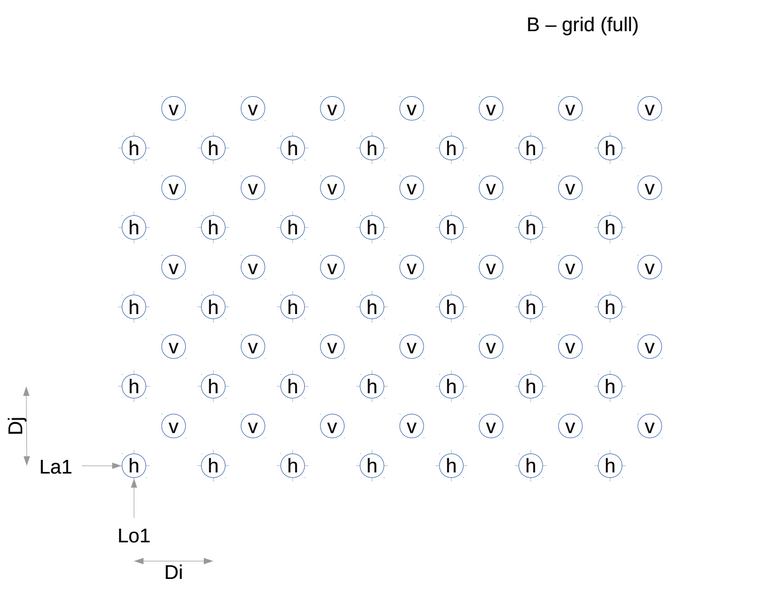
\includegraphics[width=1.58819in,height=1.39028in]{../tex/extracted-media/media/image1.png}

(a) Triangles (i) (pressure, temperature, ...)

(b) Quadrilaterals (l) (wind velocity ...)

(c) Hexagons (or pentagons, respectively) (v) (vorticity, ...)
\end{quote}

\emph{\textbf{Grid definition template 3.110 -- equatorial azimuthal equidistant projection}}

Octet No. Contents

15 Shape of the Earth (see Code table 3.2)

16 Scale factor of radius of spherical Earth

17--20 Scaled value of radius of spherical Earth

21 Scale factor of major axis of oblate spheroid Earth

22--25 Scaled value of major axis of oblate spheroid Earth

26 Scale factor of minor axis of oblate spheroid Earth

27--30 Scaled value of minor axis of oblate spheroid Earth

31--34 Nx -- number of points along x-axis

35--38 Ny -- number of points along y-axis

39--42 La1 -- latitude of tangency point (centre of grid)

43--46 Lo1 -- longitude of tangency point

47 Resolution and component flags (see Flag table 3.3)

48--51 Dx -- x-direction grid length in units of 10\textsuperscript{--3} m as measured at the point of the axis

52--55 Dy -- y-direction grid length in units of 10\textsuperscript{--3} m as measured at the point of the axis

56 Projection centre flag

57 Scanning mode (see Flag table 3.4)

Note: A scaled value of radius of spherical Earth, or major or minor axis of oblate spheroid Earth, is derived by applying the appropriate scale factor to the value expressed in metres.

\emph{\textbf{Grid definition template 3.120 -- azimuth-range projection}}

Octet No. Contents

15--18 Nb -- number of data bins along radials (see Note)

19--22 Nr -- number of radials

23--26 La1 -- latitude of centre point

27--30 Lo1 -- longitude of centre point

31--34 Dx -- spacing of bins along radials

35--38 Dstart -- offset from origin to inner bound

\emph{(continued)}

\emph{\\
(Grid definition template 3.120 -- continued)}

Octet No. Contents

39 Scanning mode (flags -- see Flag table 3.4)

\emph{40--(39+4Nr) For each of Nr radials}

(40+4(X--1))--(41+4(X--1)) Azi -- starting azimuth, degrees x 10 (degrees as north)

(42+4(X--1))--(43+4(X--1)) Adelta -- azimuthal width, degrees x 100 (+ clockwise, -- counterclockwise),\\
with X = 1 to Nr

Note: A data bin is a data point representing the volume centred on it.

\emph{\textbf{Grid definition template 3.140}} -- \emph{\textbf{Lambert azimuthal equal area projection}}

Octet No. Contents

15 Shape of the Earth (see Code table 3.2)

16 Scale factor of radius of spherical Earth

17--20 Scaled value of radius of spherical Earth

21 Scale factor of major axis of oblate spheroid Earth

22-25 Scaled value of major axis of oblate spheroid Earth

26 Scale factor of minor axis of oblate spheroid Earth

27--30 Scaled value of minor axis of oblate spheroid Earth

31--34 Nx -- number of points along the x-axis

35--38 Ny -- number of points along the y-axis

39--42 La1 -- latitude of first grid point

43--46 Lo1 -- longitude of first grid point

47--50 Standard parallel

51--54 Central longitude

55 Resolution and component flags (see Flag table 3.3)

56--59 Dx -- x-direction grid length (see Note)

60--63 Dy -- y-direction grid length (see Note)

64 Scanning mode (see Flag table 3.4)

Note: Grid lengths are in units of 10\textsuperscript{--3} m, at the latitude specified by the standard parallel.

\emph{\textbf{Grid definition template 3.1000 -- cross-section grid with points equally spaced on the horizontal}}

Preliminary note: This template is simply experimental, was not validated at the time of publication and should be used only for bilateral previously agreed tests.

Octet No. Contents

15 Shape of the Earth (see Code table 3.2)

16 Scale factor of radius of spherical Earth

17--20 Scaled value of radius of spherical Earth

21 Scale factor of major axis of oblate spheroid Earth

22--25 Scaled value of major axis of oblate spheroid Earth

26 Scale factor of minor axis of oblate spheroid Earth

27--30 Scaled value of minor axis of oblate spheroid Earth

31--34 Number of horizontal points

35--38 Basic angle of the initial production domain (see Note 1)

39--42 Subdivisions of basic angle used to define extreme longitudes and latitudes (see Note 1)

43--46 La1 -- latitude of first grid point (see Note 1)

\emph{(continued)}

\emph{\\
(Grid definition template 3.1000 -- continued)}

Octet No. Contents

47--50 Lo1 -- longitude of first grid point (see Note 1)

51 Scanning mode (flags -- see Flag table 3.4)

52--55 La2 -- latitude of last grid point (see Note 1)

56--59 Lo2 -- longitude of last grid point (see Note 1)

60 Type of horizontal line (see Code table 3.20)

61--62 Number of vertical points

63 Physical meaning of vertical coordinate (see Code table 3.15)

64 Vertical dimension coordinate values definition (see Code table 3.21)

65--66 NC -- number of coefficients or values used to specify vertical coordinates

67--(66+NCx4) Coefficients to define vertical dimension coordinate values in functional form, or the explicit\\
coordinate values (IEEE 32-bit floating-point values)

Notes:

(1) Basic angle of the initial production domain and subdivisions of this basic angle are provided to manage cases where the recommended unit of 10\textsuperscript{--6} degrees is not applicable to describe the extreme longitudes and latitudes. For these last descriptors, the unit is equal to the ratio of the basic angle and the subdivisions number.

For ordinary cases, zero and missing values should be coded, equivalent to respective values of 1 and 10\textsuperscript{6} (10\textsuperscript{--6} degrees unit).

(2) A scaled value of radius of spherical Earth, or major or minor axis of oblate spheroid Earth, is derived by applying the appropriate scale factor to the value expressed in metres.

\textbf{\\
}

\emph{\textbf{Grid definition template 3.1100 -- Hovmöller diagram grid with points equally spaced on the\\
horizontal}}

Preliminary note: This template is simply experimental, was not validated at the time of publication and should be used only for bilateral previously agreed tests.

Octet No. Contents

15 Shape of the Earth (see Code table 3.2)

16 Scale factor of radius of spherical Earth

17--20 Scaled value of radius of spherical Earth

21 Scale factor of major axis of oblate spheroid Earth

22--25 Scaled value of major axis of oblate spheroid Earth

26 Scale factor of minor axis of oblate spheroid Earth

27--30 Scaled value of minor axis of oblate spheroid Earth

31--34 Number of horizontal points

35--38 Basic angle of the initial production domain (see Note 1)

39--42 Subdivisions of basic angle used to define extreme longitudes and latitudes (see Note 1)

43--46 La1 -- latitude of first grid point (see Note 1)

47--50 Lo1 -- longitude of first grid point (see Note 1)

51 Scanning mode (flags -- see Flag table 3.4)

52--55 La2 -- latitude of last grid point (see Note 1)

56--59 Lo2 -- longitude of last grid point (see Note 1)

60 Type of horizontal line (see Code table 3.20)

61--64 NT -- number of time steps

65 Unit of offset from reference time (see Code table 4.4)

66--69 Offset from reference of first time (negative value when first bit set)

70 Type of time increment (see Code table 4.11)

71 Unit of time increment (see Code table 4.4)

72--75 Time increment (negative value when first bit set)

\emph{76--82 Last date/time}

76--77 Year

78 Month

79 Day

80 Hour

81 Minute

82 Second

Notes:

(1) Basic angle of the initial production domain and subdivisions of this basic angle are provided to manage cases where the recommended unit of 10\textsuperscript{--6} degrees is not applicable to describe the extreme longitudes and latitudes. For these last descriptors, the unit is equal to the ratio of the basic angle and the subdivisions number.

For ordinary cases, zero and missing values should be coded, equivalent to respective values of 1 and 10\textsuperscript{6} (10\textsuperscript{--6} degrees unit).

(2) A scaled value of radius of spherical Earth, or major or minor axis of oblate spheroid Earth, is derived by applying the appropriate scale factor to the value expressed in metres.

\emph{\textbf{Grid definition template 3.1200 -- time section grid}}

Preliminary note: This template is simply experimental, was not validated at the time of publication and should be used only for bilateral previously agreed tests.

Octet No. Contents

15--18 NT -- number of time steps

19 Unit of offset from reference time (see Code table 4.4)

20--23 Offset from reference of first time (negative value when first bit set)

24 Type of time increment (see Code table 4.11)

25 Unit of time increment (see Code table 4.4)

26--29 Time increment (negative value when first bit set)

\emph{30--36 Last date/time}

30--31 Year

32 Month

33 Day

34 Hour

35 Minute

36 Second

37--38 Number of vertical points

39 Physical meaning of vertical coordinate (see Code table 3.15)

40 Vertical dimension coordinate values definition (see Code table 3.21)

41--42 NC -- number of coefficients or values used to specify vertical coordinates

43--(42+NCx4) Coefficients to define vertical dimension coordinate values in functional form, or the explicit\\
coordinate values (IEEE 32-bit floating-point values)

\_\_\_\_\_\_\_\_\_\_\_

\textbf{TEMPLATE DEFINITIONS USED IN SECTION 4}

\emph{\textbf{Product definition template 4.0 -- analysis or forecast at a horizontal level or in a horizontal layer\\
at a point in time}}

Octet No. Contents

10 Parameter category (see Code table 4.1)

11 Parameter number (see Code table 4.2)

12 Type of generating process (see Code table 4.3)

13 Background generating process identifier (defined by originating centre)

14 Analysis or forecast generating process identifier (defined by originating centre)

15--16 Hours of observational data cut-off after reference time (see Note)

17 Minutes of observational data cut-off after reference time

18 Indicator of unit of time range (see Code table 4.4)

19--22 Forecast time in units defined by octet 18

23 Type of first fixed surface (see Code table 4.5)

24 Scale factor of first fixed surface

25--28 Scaled value of first fixed surface

29 Type of second fixed surface (see Code table 4.5)

30 Scale factor of second fixed surface

31--34 Scaled value of second fixed surface

Note: Hours greater than 65534 will be coded as 65534.

\emph{\textbf{Product definition template 4.1 -- individual ensemble forecast, control and perturbed, at a\\
horizontal level or in a horizontal layer at a point in time}}

Octet No. Contents

10 Parameter category (see Code table 4.1)

11 Parameter number (see Code table 4.2)

12 Type of generating process (see Code table 4.3)

13 Background generating process identifier (defined by originating centre)

14 Forecast generating process identifier (defined by originating centre)

15--16 Hours after reference time of data cut-off (see Note)

17 Minutes after reference time of data cut-off

18 Indicator of unit of time range (see Code table 4.4)

19--22 Forecast time in units defined by octet 18

23 Type of first fixed surface (see Code table 4.5)

24 Scale factor of first fixed surface

25--28 Scaled value of first fixed surface

29 Type of second fixed surface (see Code table 4.5)

30 Scale factor of second fixed surface

31--34 Scaled value of second fixed surface

35 Type of ensemble forecast (see Code table 4.6)

36 Perturbation number

37 Number of forecasts in ensemble

Note: Hours greater than 65534 will be coded as 65534.

\emph{\textbf{Product definition template 4.2 -- derived forecasts based on all ensemble members at\\
a horizontal level or in a horizontal layer at a point in time}}

Octet No. Contents

10 Parameter category (see Code table 4.1)

11 Parameter number (see Code table 4.2)

12 Type of generating process (see Code table 4.3)

13 Background generating process identifier (defined by originating centre)

14 Forecast generating process identifier (defined by originating centre)

15--16 Hours after reference time of data cut-off (see Note)

17 Minutes after reference time of data cut-off

18 Indicator of unit of time range (see Code table 4.4)

19--22 Forecast time in units defined by octet 18

23 Type of first fixed surface (see Code table 4.5)

24 Scale factor of first fixed surface

25--28 Scaled value of first fixed surface

29 Type of second fixed surface (see Code table 4.5)

30 Scale factor of second fixed surface

31--34 Scaled value of second fixed surface

35 Derived forecast (see Code table 4.7)

36 Number of forecasts in ensemble

Note: Hours greater than 65534 will be coded as 65534.

\emph{\textbf{Product definition template 4.3 -- derived forecasts based on a cluster of ensemble members over a rectangular area at a horizontal level or in a horizontal layer at a point in time}}

Octet No. Contents

10 Parameter category (see Code table 4.1)

11 Parameter number (see Code table 4.2)

12 Type of generating process (see Code table 4.3)

13 Background generating process identifier (defined by originating centre)

14 Forecast generating process identifier (defined by originating centre)

15--16 Hours after reference time of data cut-off (see Note)

17 Minutes after reference time of data cut-off

18 Indicator of unit of time range (see Code table 4.4)

19--22 Forecast time in units defined by octet 18

23 Type of first fixed surface (see Code table 4.5)

24 Scale factor of first fixed surface

25--28 Scaled value of first fixed surface

29 Type of second fixed surface (see Code table 4.5)

30 Scale factor of second fixed surface

31--34 Scaled value of second fixed surface

35 Derived forecast (see Code table 4.7)

36 Number of forecasts in the ensemble (N)

37 Cluster identifier

38 Number of cluster to which the high-resolution control belongs

39 Number of cluster to which the low-resolution control belongs

\emph{(continued)}

\emph{\\
(Product definition template 4.3 -- continued)}

Octet No. Contents

40 Total number of clusters

41 Clustering method (see Code table 4.8)

42--45 Northern latitude of cluster domain

46--49 Southern latitude of cluster domain

50--53 Eastern longitude of cluster domain

54--57 Western longitude of cluster domain

58 N\textsubscript{c} -- number of forecasts in the cluster

59 Scale factor of standard deviation in the cluster

60--63 Scaled value of standard deviation in the cluster

64 Scale factor of distance of the cluster from ensemble mean

65--68 Scaled value of distance of the cluster from ensemble mean

69--(68+N\textsubscript{c}) List of N\textsubscript{c} ensemble forecast numbers (N\textsubscript{c} is given in octet 58)

Note: Hours greater than 65534 will be coded as 65534.

\emph{\textbf{Product definition template 4.4 -- derived forecasts based on a cluster of ensemble members\\
over a circular area at a horizontal level or in a horizontal layer\\
at a point in time}}

Octet No. Contents

10 Parameter category (see Code table 4.1)

11 Parameter number (see Code table 4.2)

12 Type of generating process (see Code table 4.3)

13 Background generating process identifier (defined by originating centre)

14 Forecast generating process identifier (defined by originating centre)

15--16 Hours after reference time of data cut-off (see Note)

17 Minutes after reference time of data cut-off

18 Indicator of unit of time range (see Code table 4.4)

19--22 Forecast time in units defined by octet 18

23 Type of first fixed surface (see Code table 4.5)

24 Scale factor of first fixed surface

25--28 Scaled value of first fixed surface

29 Type of second fixed surface (see Code table 4.5)

30 Scale factor of second fixed surface

31--34 Scaled value of second fixed surface

35 Derived forecast (see Code table 4.7)

36 Number of forecasts in the ensemble (N)

37 Cluster identifier

38 Number of cluster to which the high-resolution control belongs

39 Number of cluster to which the low-resolution control belongs

40 Total number of clusters

41 Clustering method (see Code table 4.8)

42--45 Latitude of central point in cluster domain

46--49 Longitude of central point in cluster domain

50--53 Radius of cluster domain

54 N\textsubscript{c} -- number of forecasts in the cluster

\emph{(continued)}

\emph{\\
(Product definition template 4.4 -- continued)}

Octet No. Contents

55 Scale factor of standard deviation in the cluster

56--59 Scaled value of standard deviation in the cluster

60 Scale factor of distance of the cluster from ensemble mean

61--64 Scaled value of distance of the cluster from ensemble mean

65--(64+N\textsubscript{c}) List of N\textsubscript{c} ensemble forecast numbers (N\textsubscript{c} is given in octet 54)

Note: Hours greater than 65534 will be coded as 65534.

\emph{\textbf{Product definition template 4.5 -- probability forecasts at a horizontal level or in a horizontal layer\\
at a point in time}}

Octet No. Contents

10 Parameter category (see Code table 4.1)

11 Parameter number (see Code table 4.2)

12 Type of generating process (see Code table 4.3)

13 Background generating process identifier (defined by originating centre)

14 Forecast generating process identifier (defined by originating centre)

15--16 Hours after reference time of data cut-off (see Note)

17 Minutes after reference time of data cut-off

18 Indicator of unit of time range (see Code table 4.4)

19--22 Forecast time in units defined by octet 18

23 Type of first fixed surface (see Code table 4.5)

24 Scale factor of first fixed surface

25--28 Scaled value of first fixed surface

29 Type of second fixed surface (see Code table 4.5)

30 Scale factor of second fixed surface

31--34 Scaled value of second fixed surface

35 Forecast probability number

36 Total number of forecast probabilities

37 Probability type (see Code table 4.9)

38 Scale factor of lower limit

39--42 Scaled value of lower limit

43 Scale factor of upper limit

44--47 Scaled value of upper limit

Note: Hours greater than 65534 will be coded as 65534.

\emph{\textbf{Product definition template 4.6 -- percentile forecasts at a horizontal level or in a horizontal layer\\
at a point in time}}

Octet No. Contents

10 Parameter category (see Code table 4.1)

11 Parameter number (see Code table 4.2)

12 Type of generating process (see Code table 4.3)

13 Background generating process identifier (defined by originating centre)

14 Forecast generating process identifier (defined by originating centre)

\emph{(continued)}

\emph{\\
(Product definition template 4.6 -- continued)}

Octet No. Contents

15--16 Hours after reference time of data cut-off (see Note)

17 Minutes after reference time of data cut-off

18 Indicator of unit of time range (see Code table 4.4)

19--22 Forecast time in units defined by octet 18

23 Type of first fixed surface (see Code table 4.5)

24 Scale factor of first fixed surface

25--28 Scaled value of first fixed surface

29 Type of second fixed surface (see Code table 4.5)

30 Scale factor of second fixed surface

31--34 Scaled value of second fixed surface

35 Percentile value (from 100\% to 0\%)

Note: Hours greater than 65534 will be coded as 65534.

\emph{\textbf{Product definition template 4.7 -- analysis or forecast error at a horizontal level or in a horizontal\\
layer at a point in time}}

Octet No. Contents

10 Parameter category (see Code table 4.1)

11 Parameter number (see Code table 4.2)

12 Type of generating process (see Code table 4.3)

13 Background generating process identifier (defined by originating centre)

14 Analysis or forecast generating process identifier (defined by originating centre)

15--16 Hours after reference time of data cut-off (see Note 1)

17 Minutes after reference time of data cut-off

18 Indicator of unit of time range (see Code table 4.4)

19--22 Forecast time in units defined by octet 18

23 Type of first fixed surface (see Code table 4.5)

24 Scale factor of first fixed surface

25--28 Scaled value of first fixed surface

29 Type of second fixed surface (see Code table 4.5)

30 Scale factor of second fixed surface

31--34 Scaled value of second fixed surface

Notes:

(1) Hours greater than 65534 will be coded as 65534.

(2) This template should not be used. Product definition template 4.0 should be used instead.

\emph{\textbf{Product definition template 4.8 -- average, accumulation and/or extreme values or other\\
statistically processed values at a horizontal level or in a horizontal layer in a continuous or non-continuous time\\
interval}}

Octet No. Contents

10 Parameter category (see Code table 4.1)

11 Parameter number (see Code table 4.2)

12 Type of generating process (see Code table 4.3)

13 Background generating process identifier (defined by originating centre)

\emph{(continued)}

\emph{\\
(Product definition template 4.8 -- continued)}

Octet No. Contents

14 Analysis or forecast generating process identifier (defined by originating centre)

15--16 Hours after reference time of data cut-off (see Note 1)

17 Minutes after reference time of data cut-off

18 Indicator of unit of time range (see Code table 4.4)

19--22 Forecast time in units defined by octet 18 (see Note 2)

23 Type of first fixed surface (see Code table 4.5)

24 Scale factor of first fixed surface

25--28 Scaled value of first fixed surface

29 Type of second fixed surface (see Code table 4.5)

30 Scale factor of second fixed surface

31--34 Scaled value of second fixed surface

35--36 Year

37 Month

38 Day Time of end of overall time interval

39 Hour

40 Minute

41 Second

42 n -- number of time range specifications describing the time intervals used to calculate the\\
statistically processed field

43--46 Total number of data values missing in statistical process

\emph{47--58 Specification of the outermost (or only) time range over which statistical}\\
\emph{processing is done}

47 Statistical process used to calculate the processed field from the field at each time incre-\\
ment during the time range (see Code table 4.10)

48 Type of time increment between successive fields used in the statistical processing (see\\
Code table 4.11)

49 Indicator of unit of time for time range over which statistical processing is done (see Code\\
table 4.4)

50--53 Length of the time range over which statistical processing is done, in units defined by the\\
previous octet

54 Indicator of unit of time for the increment between the successive fields used (see Code\\
table 4.4)

55--58 Time increment between successive fields, in units defined by the previous octet (see Notes 3\\
and 4)

\emph{59--nn These octets are included only if n \textgreater{} 1, where nn = 46 + 12 x n}

59--70 As octets 47 to 58, next innermost step of processing

71--nn Additional time range specifications, included in accordance with the value of n. Contents\\
as octets 47 to 58, repeated as necessary

Notes:

(1) Hours greater than 65534 will be coded as 65534.

(2) The reference time in section 1 and the forecast time together define the beginning of the overall time interval.

(3) An increment of zero means that the statistical processing is the result of a continuous (or near continuous) process, not the processing of a number of discrete samples. Examples of such continuous processes are the temperatures measured by analogue maximum and minimum thermometers or thermographs, and the rainfall measured by a raingauge.

(4) The reference and forecast times are successively set to their initial values plus or minus the increment, as defined by the type of time increment (one of octets 48, 60, 72, ...). For all but the innermost (last) time range, the next inner range is then processed using these reference and forecast times as the initial reference and forecast times.

\emph{\textbf{\\
}}

\emph{\textbf{Product definition template 4.9 -- probability forecasts at a horizontal level or in a horizontal layer}}

\emph{\textbf{in a continuous or non-continuous time interval}}

Octet No. Contents

10 Parameter category (see Code table 4.1)

11 Parameter number (see Code table 4.2)

12 Type of generating process (see Code table 4.3)

13 Background generating process identifier (defined by originating centre)

14 Forecast generating process identifier (defined by originating centre)

15--16 Hours after reference time of data cut-off (see Note 1)

17 Minutes after reference time of data cut-off

18 Indicator of unit of time range (see Code table 4.4)

19--22 Forecast time in units defined by octet 18 (see Note 2)

23 Type of first fixed surface (see Code table 4.5)

24 Scale factor of first fixed surface

25--28 Scaled value of first fixed surface

29 Type of second fixed surface (see Code table 4.5)

30 Scale factor of second fixed surface

31--34 Scaled value of second fixed surface

35 Forecast probability number

36 Total number of forecast probabilities

37 Probability type (see Code table 4.9)

38 Scale factor of lower limit

39--42 Scaled value of lower limit

43 Scale factor of upper limit

44--47 Scaled value of upper limit

48--49 Year of end of overall time interval

50 Month of end of overall time interval

51 Day of end of overall time interval

52 Hour of end of overall time interval

53 Minute of end of overall time interval

54 Second of end of overall time interval

55 n -- number of time range specifications describing the time intervals used to calculate the\\
statistically processed field

56--59 Total number of data values missing in the statistical process

\emph{60--71 Specification of the outermost (or only) time range over which statistical}\\
\emph{processing is done}

60 Statistical process used to calculate the processed field from the field at each time incre-\\
ment during the time range (see Code table 4.10)

61 Type of time increment between successive fields used in the statistical processing (see\\
Code table 4.11)

62 Indicator of unit of time for time range over which statistical processing is done (see Code\\
table 4.4)

63--66 Length of the time range over which statistical processing is done, in units defined by the\\
previous octet

67 Indicator of unit of time for the increment between the successive fields used (see Code\\
table 4.4)

68--71 Time increment between successive fields, in units defined by the previous octet (see\\
Notes 3 and 4)

\emph{(continued)}

\emph{\\
(Product definition template 4.9 -- continued)}

Octet No. Contents

\emph{72--nn These octets are included only if n \textgreater{} 1, where nn = 59 + 12 x n}

72--83 As octets 60 to 71, next innermost step of processing

84--nn Additional time range specifications, included in accordance with the value of n. Contents\\
as octets 60 to 71, repeated as necessary.

Notes:

(1) Hours greater than 65534 will be coded as 65534.

(2) The reference time in section 1 and the forecast time together define the beginning of the overall time interval.

(3) An increment of zero means that the statistical processing is the result of a continuous (or near continuous) process, not the processing of a number of discrete samples. Examples of such continuous processes are the temperatures measured by analogue maximum and minimum thermometers or thermographs, and the rainfall measured by a raingauge.

(4) The reference and forecast times are successively set to their initial values plus or minus the increment, as defined by the type of time increment (one of octets 46, 58, 70, ...). For all but the innermost (last) time range, the next inner range is then processed using these reference and forecast times as the initial reference and forecast times.

\emph{\textbf{Product definition template 4.10 -- percentile forecasts at a horizontal level or in a horizontal\\
layer in a continuous or non-continuous time interval}}

Preliminary note: This template was not validated at the time of publication and should be used with caution. Please report any use to the WMO Secretariat (Observing and Information Systems Department) to assist for validation.

Octet No. Contents

10 Parameter category (see Code table 4.1)

11 Parameter number (see Code table 4.2)

12 Type of generating process (see Code table 4.3)

13 Background generating process identifier (defined by originating centre)

14 Forecast generating process identifier (defined by originating centre)

15--16 Hours after reference time of data cut-off (see Note 1)

17 Minutes after reference time for data cut-off

18 Indicator of unit of time range (see Code table 4.4)

19--22 Forecast time in units defined by previous octet (see Note 2)

23 Type of first fixed surface (see Code table 4.5)

24 Scale factor of first fixed surface

25--28 Scaled value of first fixed surface

29 Type of second fixed surface (see Code table 4.5)

30 Scale factor of second fixed surface

31--34 Scaled value of second fixed surface

35 Percentile value (from 100\% to 0\%)

36--37 Year of end of overall time interval

38 Month of end of overall time interval

39 Day of end of overall time interval

40 Hour of end of overall time interval

41 Minute of end of overall time interval

42 Second of end of overall time interval

43 n -- number of time range specifications describing the time intervals used to calculate the\\
statistically processed field

44--47 Total number of data values missing in the statistical process

\emph{(continued)}

\emph{\\
(Product definition template 4.10 -- continued)}

Octet No. Contents

\emph{48--59 Specification of the outermost (or only) time range over which statistical}\\
\emph{processing is done}

48 Statistical process used to calculate the processed field from the field at each time incre-\\
ment during the time range (see Code table 4.10)

49 Type of time increment between successive fields used in the statistical processing (see\\
Code table 4.11)

50 Indicator of unit of time for time range over which statistical processing is done (see Code\\
table 4.4)

51--54 Length of the time range over which statistical processing is done, in units defined by the\\
previous octet

55 Indicator of unit of time for the increment between the successive fields used (see Code\\
table 4.4)

56--59 Time increment between successive fields, in units defined by the previous octet (see\\
Note 3)

\emph{60--nn These octets are included only if n \textgreater{} 1, where nn = 47 + 12 x n}

60--71 As octets 48--59, next innermost step of processing

72--nn Additional time range specifications, included in accordance with the value of n. Contents\\
as octets 48 to 59, repeated as necessary.

Notes:

(1) Hours greater than 65534 will be coded as 65534.

(2) The reference time in section 1 and the forecast time together define the beginning of the overall time interval.

(3) An increment of zero means that the statistical processing is the result of a continuous (or near continuous) process, not the processing of a number of discrete samples. Examples of such continuous processes are the temperatures measured by analogue maximum and minimum thermometers or thermographs, and the rainfall measured by raingauge.

\emph{\textbf{Product definition template 4.11 -- individual ensemble forecast, control and perturbed, at a\\
horizontal level or in a horizontal layer in a continuous or non-\\
continuous time interval}}

Octet No. Contents

10 Parameter category (see Code table 4.1)

11 Parameter number (see Code table 4.2)

12 Type of generating process (see Code table 4.3)

13 Background generating process identifier (defined by originating centre)

14 Forecast generating process identifier (defined by originating centre)

15--16 Hours after reference time of data cut-off (see Note 1)

17 Minutes after reference time of data cut-off

18 Indicator of unit of time range (see Code table 4.4)

19--22 Forecast time in units defined by octet 18 (see Note 2)

23 Type of first fixed surface (see Code table 4.5)

24 Scale factor of first fixed surface

25--28 Scaled value of first fixed surface

29 Type of second fixed surface (see Code table 4.5)

30 Scale factor of second fixed surface

31--34 Scaled value of second fixed surface

35 Type of ensemble forecast (see Code table 4.6)

36 Perturbation number

\emph{(continued)}

\emph{\\
(Product definition template 4.11 -- continued)}

Octet No. Contents

37 Number of forecasts in ensemble

38--39 Year of end of overall time interval

40 Month of end of overall time interval

41 Day of end of overall time interval

42 Hour of end of overall time interval

43 Minute of end of overall time interval

44 Second of end of overall time interval

45 n -- number of time range specifications describing the time intervals used to calculate the\\
statistically processed field

46--49 Total number of data values missing in statistical process

\emph{50--61 Specification of the outermost (or only) time range over which statistical}\\
\emph{processing is done}

50 Statistical process used to calculate the processed field from the field at each time incre-\\
ment during the time range (see Code table 4.10)

51 Type of time increment between successive fields used in the statistical processing (see\\
Code table 4.11)

52 Indicator of unit of time for time range over which statistical processing is done (see Code\\
table 4.4)

53--56 Length of the time range over which statistical processing is done, in units defined by the\\
previous octet

57 Indicator of unit of time for the increment between the successive fields used (see Code\\
table 4.4)

58--61 Time increment between successive fields, in units defined by the previous octet (see\\
Notes 3 and 4)

\emph{62--nn These octets are included only if n \textgreater{} 1, where nn = 49 + 12 x n}

62--73 As octets 50 to 61, next innermost step of processing

74--nn Additional time range specifications, included in accordance with the value of n. Contents\\
as octets 50 to 61, repeated as necessary

Notes:

(1) Hours greater than 65534 will be coded as 65534.

(2) The reference time in section 1 and the forecast time together define the beginning of the overall time interval.

(3) An increment of zero means that the statistical processing is the result of a continuous (or near continuous) process, not the processing of a number of discrete samples. Examples of such continuous processes are the temperatures measured by analogue maximum and minimum thermometers or thermographs, and the rainfall measured by a raingauge.

(4) The reference and forecast times are successively set to their initial values plus or minus the increment, as defined by the type of time increment (one of octets 51, 63, 75, ...). For all but the innermost (last) time range, the next inner range is then processed using these reference and forecast times as the initial reference and forecast times.

\emph{\textbf{Product definition template 4.12 -- derived forecasts based on all ensemble members at a\\
horizontal level or in a horizontal layer in a continuous or non-\\
continuous time interval}}

Octet No. Contents

10 Parameter category (see Code table 4.1)

11 Parameter number (see Code table 4.2)

12 Type of generating process (see Code table 4.3)

13 Background generating process identifier (defined by originating centre)

\emph{(continued)}

\emph{\\
(Product definition template 4.12 -- continued)}

Octet No. Contents

14 Forecast generating process identifier (defined by originating centre)

15--16 Hours after reference time of data cut-off (see Note 1)

17 Minutes after reference time of data cut-off

18 Indicator of unit of time range (see Code table 4.4)

19--22 Forecast time in units defined by octet 18 (see Note 2)

23 Type of first fixed surface (see Code table 4.5)

24 Scale factor of first fixed surface

25--28 Scaled value of first fixed surface

29 Type of second fixed surface (see Code table 4.5)

30 Scale factor of second fixed surface

31--34 Scaled value of second fixed surface

35 Derived forecast (see Code table 4.7)

36 Number of forecasts in the ensemble (N)

37--38 Year of end of overall time interval

39 Month of end of overall time interval

40 Day of end of overall time interval

41 Hour of end of overall time interval

42 Minute of end of overall time interval

43 Second of end of overall time interval

44 n -- number of time range specifications describing the time intervals used to calculate the\\
statistically processed field

45--48 Total number of data values missing in statistical process

\emph{49--60 Specification of the outermost (or only) time range over which statistical}\\
\emph{processing is done}

49 Statistical process used to calculate the processed field from the field at each time incre-\\
ment during the time range (see Code table 4.10)

50 Type of time increment between successive fields used in the statistical processing (see\\
Code table 4.11)

51 Indicator of unit of time for time range over which statistical processing is done (see Code\\
table 4.4)

52--55 Length of the time range over which statistical processing is done, in units defined by the\\
previous octet

56 Indicator of unit of time for the increment between the successive fields used (see Code\\
table 4.4)

57--60 Time increment between successive fields, in units defined by the previous octet (see\\
Notes 3 and 4)

\emph{61--nn These octets are included only if n \textgreater{} 1, where nn = 48 + 12 x n}

61--72 As octets 49 to 60, next innermost step of processing

73--nn Additional time range specifications, included in accordance with the value of n. Contents\\
as octets 49 to 60, repeated as necessary

Notes:

(1) Hours greater than 65534 will be coded as 65534.

(2) The reference time in section 1 and the forecast time together define the beginning of the overall time interval.

(3) An increment of zero means that the statistical processing is the result of a continuous (or near continuous) process, not the processing of a number of discrete samples. Examples of such continuous processes are the temperatures measured by analogue maximum and minimum thermometers or thermographs, and the rainfall measured by a raingauge.

(4) The reference and forecast times are successively set to their initial values plus or minus the increment, as defined by the type of time increment (one of octets 50, 62, 74, ...). For all but the innermost (last) time range, the next inner range is then processed using these reference and forecast times as the initial reference and forecast times.

\emph{\textbf{Product definition template 4.13 -- derived forecasts based on a cluster of ensemble members\\
over a rectangular area at a horizontal level or in a horizontal\\
layer in a continuous or non-continuous time interval}}

Octet No. Contents

10 Parameter category (see Code table 4.1)

11 Parameter number (see Code table 4.2)

12 Type of generating process (see Code table 4.3)

13 Background generating process identifier (defined by originating centre)

14 Forecast generating process identifier (defined by originating centre)

15--16 Hours after reference time of data cut-off (see Note 1)

17 Minutes after reference time of data cut-off

18 Indicator of unit of time range (see Code table 4.4)

19--22 Forecast time in units defined by octet 18 (see Note 2)

23 Type of first fixed surface (see Code table 4.5)

24 Scale factor of first fixed surface

25--28 Scaled value of first fixed surface

29 Type of second fixed surface (see Code table 4.5)

30 Scale factor of second fixed surface

31--34 Scaled value of second fixed surface

35 Derived forecast (see Code table 4.7)

36 Number of forecasts in the ensemble (N)

37 Cluster identifier

38 Number of cluster to which the high-resolution control belongs

39 Number of cluster to which the low-resolution control belongs

40 Total number of clusters

41 Clustering method (see Code table 4.8)

42--45 Northern latitude of cluster domain

46--49 Southern latitude of cluster domain

50--53 Eastern longitude of cluster domain

54--57 Western longitude of cluster domain

58 N\textsubscript{C} -- number of forecasts in the cluster

59 Scale factor of standard deviation in the cluster

60--63 Scaled value of standard deviation in the cluster

64 Scale factor of distance of the cluster from ensemble mean

65--68 Scaled value of distance of the cluster from ensemble mean

69--70 Year of end of overall time interval

71 Month of end of overall time interval

72 Day of end of overall time interval

73 Hour of end of overall time interval

74 Minute of end of overall time interval

75 Second of end of overall time interval

76 n -- number of time range specifications describing the time intervals used to calculate the\\
statistically processed field

77--80 Total number of data values missing in statistical process

\emph{81--92 Specification of the outermost (or only) time range over which statistical}\\
\emph{processing is done}

81 Statistical process used to calculate the processed field from the field at each time incre-\\
ment during the time range (see Code table 4.10)

\emph{(continued)}

\emph{\\
(Product definition template 4.13 -- continued)}

Octet No. Contents

82 Type of time increment between successive fields used in the statistical processing (see\\
Code table 4.11)

83 Indicator of unit of time for time range over which statistical processing is done (see Code\\
table 4.4)

84--87 Length of the time range over which statistical processing is done, in units defined by the\\
previous octet

88 Indicator of unit of time for the increment between the successive fields used (see Code\\
table 4.4)

89--92 Time increment between successive fields, in units defined by the previous octet (see\\
Notes 3 and 4)

\emph{93--nn These octets are included only if n \textgreater{} 1, where nn = 80 + 12 x n}

93--104 As octets 81 to 92, next innermost step of processing

105--nn Additional time range specifications, included in accordance with the value of n. Contents\\
as octets 81 to 92, repeated as necessary

(nn+1)--(nn+N\textsubscript{C}) List of N\textsubscript{C} ensemble forecast numbers (N\textsubscript{C} is given in octet 58)

Notes:

(1) Hours greater than 65534 will be coded as 65534.

(2) The reference time in section 1 and the forecast time together define the beginning of the overall time interval.

(3) An increment of zero means that the statistical processing is the result of a continuous (or near continuous) process, not the processing of a number of discrete samples. Examples of such continuous processes are the temperatures measured by analogue maximum and minimum thermometers or thermographs, and the rainfall measured by a raingauge.

(4) The reference and forecast times are successively set to their initial values plus or minus the increment, as defined by the type of time increment (one of octets 82, 94, 106,....). For all but the innermost (last) time range, the next inner range is then processed using these reference and forecast times as the initial reference and forecast times.

\emph{\textbf{Product definition template 4.14 -- derived forecasts based on a cluster of ensemble members\\
over a circular area at a horizontal level or in a horizontal layer\\
in a continuous or non-continuous time interval}}

Octet No. Contents

10 Parameter category (see Code table 4.1)

11 Parameter number (see Code table 4.2)

12 Type of generating process (see Code table 4.3)

13 Background generating process identifier (defined by originating centre)

14 Forecast generating process identifier (defined by originating centre)

15--16 Hours after reference time of data cut-off (see Note 1)

17 Minutes after reference time of data cut-off

18 Indicator of unit of time range (see Code table 4.4)

19--22 Forecast time in units defined by octet 18 (see Note 2)

23 Type of first fixed surface (see Code table 4.5)

24 Scale factor of first fixed surface

25--28 Scaled value of first fixed surface

29 Type of second fixed surface (see Code table 4.5)

30 Scale factor of second fixed surface

31--34 Scaled value of second fixed surface

35 Derived forecast (see Code table 4.7)

36 Number of forecasts in the ensemble (N)

\emph{(continued)}

\emph{\\
(Product definition template 4.14 -- continued)}

Octet No. Contents

37 Cluster identifier

38 Number of cluster to which the high-resolution control belongs

39 Number of cluster to which the low-resolution control belongs

40 Total number of clusters

41 Clustering method (see Code table 4.8)

42--45 Latitude of central point in cluster domain

46--49 Longitude of central point in cluster domain

50--53 Radius of cluster domain

54 N\textsubscript{C} -- number of forecasts in the cluster

55 Scale factor of standard deviation in the cluster

56--59 Scaled value of standard deviation in the cluster

60 Scale factor of distance of the cluster from ensemble mean

61--64 Scaled value of distance of the cluster from ensemble mean

65--66 Year of end of overall time interval

67 Month of end of overall time interval

68 Day of end of overall time interval

69 Hour of end of overall time interval

70 Minute of end of overall time interval

71 Second of end of overall time interval

72 n -- number of time range specifications describing the time intervals used to calculate the\\
statistically processed field

73--76 Total number of data values missing in statistical process

\emph{77--88 Specification of the outermost (or only) time range over which statistical}\\
\emph{processing is done}

77 Statistical process used to calculate the processed field from the field at each time incre-\\
ment during the time range (see Code table 4.10)

78 Type of time increment between successive fields used in the statistical processing (see\\
Code table 4.11)

79 Indicator of unit of time for time range over which statistical processing is done (see Code\\
table 4.4)

80--83 Length of the time range over which statistical processing is done, in units defined by the\\
previous octet

84 Indicator of unit of time for the increment between the successive fields used (see Code\\
table 4.4)

85--88 Time increment between successive fields, in units defined by the previous octet (see\\
Notes 3 and 4)

\emph{89--nn These octets are included only if n \textgreater{} 1, where nn = 76 + 12 x n}

89--110 As octets 77 to 88, next innermost step of processing

111--nn Additional time range specifications, included in accordance with the value of n. Contents\\
as octets 77 to 88, repeated as necessary

(nn+1)--(nn+N\textsubscript{C}) List of N\textsubscript{C} ensemble forecast numbers (N\textsubscript{C} is given in octet 54)

Notes:

(1) Hours greater than 65534 will be coded as 65534.

(2) The reference time in section 1 and the forecast time together define the beginning of the overall time interval.

\emph{(continued)}

\emph{\\
(Product definition template 4.14 -- continued)}

(3) An increment of zero means that the statistical processing is the result of a continuous (or near continuous) process, not the processing of a number of discrete samples. Examples of such continuous processes are the temperatures measured by analogue maximum and minimum thermometers or thermographs, and the rainfall measured by a raingauge.

(4) The reference and forecast times are successively set to their initial values plus or minus the increment, as defined by the type of time increment (one of octets 78, 90, 112, ...). For all but the innermost (last) time range, the next inner range is then processed using these reference and forecast times as the initial reference and forecast times.

\emph{\textbf{Product definition template 4.15 -- average, accumulation, extreme values, or other\\
statistically processed values over a spatial area at a\\
horizontal level or in a horizontal layer at a point in time}}

Octet No. Contents

10 Parameter category (see Code table 4.1)

11 Parameter number (see Code table 4.2)

12 Type of generating process (see Code table 4.3)

13 Background generating process identifier (defined by originating centre)

14 Analysis or forecast generating process identifier (defined by originating centre)

15--16 Hours of observational data cut-off after reference time (see Note)

17 Minutes of observational data cut-off after reference time

18 Indicator of unit of time range (see Code table 4.4)

19--22 Forecast time in units defined by octet 18

23 Type of first fixed surface (see Code table 4.5)

24 Scale factor of first fixed surface

25--28 Scaled value of first fixed surface

29 Type of second fixed surface (see Code table 4.5)

30 Scale factor of second fixed surface

31--34 Scaled value of second fixed surface

35 Statistical process used within the spatial area defined by octet 36 (see Code table 4.10)

36 Type of spatial processing used to arrive at given data value from the source data (see\\
Code table 4.15)

37 Number of data points used in spatial processing defined in octet 36

Note: Hours greater than 65534 will be coded as 65534.

\emph{\textbf{\\
}}

\emph{\textbf{Product definition template 4.20 -- radar product}}

Octet No. Contents

10 Parameter category (see Code table 4.1)

11 Parameter number (see Code table 4.2)

12 Type of generating process (see Code table 4.3)

13 Number of radar sites used

14 Indicator of unit of time range

15--18 Site latitude (in 10\textsuperscript{--6} degree)

19--22 Site longitude (in 10\textsuperscript{--6} degree)

23--24 Site elevation (metres)

25--28 Site ID (alphanumeric)

29--30 Site ID (numeric)

31 Operating mode (see Code table 4.12)

32 Reflectivity calibration constant (tenths of dB)

33 Quality control indicator (see Code table 4.13)

34 Clutter filter indicator (see Code table 4.14)

35 Constant antenna elevation angle (tenths of degree true)

36--37 Accumulation interval (minutes)

38 Reference reflectivity for echo top (dB)

39--41 Range bin spacing (metres)

42--43 Radial angular spacing (tenths of degree true)

\emph{\textbf{Product definition template 4.30 -- satellite product}}

Note: This template is deprecated. Template 4.31 should be used instead.

Octet No. Contents

10 Parameter category (see Code table 4.1)

11 Parameter number (see Code table 4.2)

12 Type of generating process (see Code table 4.3)

13 Observation generating process identifier (defined by originating centres)

14 Number of contributing spectral bands (NB)

\emph{15-- Repeat the following 10 octets for each contributing band (nb = 1, NB)}

(15+10(nb--1))--(16+10(nb--1)) Satellite series of band nb (code table defined by originating/generating centre)

(17+10(nb--1))--(18+10(nb--1)) Satellite numbers of band nb (code table defined by originating/generating centre)

(19+10(nb--1)) Instrument types of band nb (code table defined by originating/generating centre)

(20+10(nb--1)) Scale factor of central wave number of band nb

(21+10(nb--1))--(24+10(nb--1)) Scaled value of central wave number of band nb (units: m\textsuperscript{--1})

Note: For ``satellite series of band nb'', ``satellite numbers of band nb'' and ``instrument types of band nb'', it is recommended to encode the values as per BUFR Code tables 0 02 020, 0 01 007 (Common Code table C--5) and 0 02 019 (Common Code table C--8), respectively.

\emph{\textbf{\\
}}

\emph{\textbf{Product definition template 4.31 -- satellite product}}

Octet No. Contents

10 Parameter category (see Code table 4.1)

11 Parameter number (see Code table 4.2)

12 Type of generating process (see Code table 4.3)

13 Observation generating process identifier (defined by originating centres)

14 Number of contributing spectral bands (NB)

\emph{15-- Repeat the following 11 octets for each contributing band (nb = 1, NB)}

(15+11(nb--1))--(16+11(nb--1)) Satellite series of band nb (code table defined by originating/generating centre)

(17+11(nb--1))--(18+11(nb--1)) Satellite numbers of band nb (code table defined by originating/generating centre)

(19+11(nb--1))--(20+11(nb--1)) Instrument types of band nb (code table defined by originating/generating centre)

(21+11(nb--1)) Scale factor of central wave number of band nb

(22+11(nb--1))--(25+11(nb--1)) Scaled value of central wave number of band nb (units: m\textsuperscript{--1})

Note: For ``satellite series of band nb'', ``satellite numbers of band nb'' and ``instrument types of band nb'', it is recommended to encode the values as per BUFR Code tables 0 02 020, 0 01 007 (Common Code table C--5) and 0 02 019 (Common Code table C--8), respectively.

\emph{\textbf{Product definition template 4.32 -- analysis or forecast at a horizontal level or in a horizontal layer\\
at a point in time for simulated (synthetic) satellite data}}

Octet No. Contents

10 Parameter category (see Code table 4.1)

11 Parameter number (see Code table 4.2)

12 Type of generating process (see Code table 4.3)

13 Background generating process identifier (defined by originating centre)

14 Analysis or forecast generating process identifier

15--16 Hours of observational data cut-off after reference time (see Note 2)

17 Minutes of observational data cut-off after reference time

18 Indicator of unit of time range (see Code table 4.4)

19--22 Forecast time in units defined by octet 18

23 Number of contributing spectral bands (NB)

\emph{24-- Repeat the following 11 octets for each contributing band (nb = 1, NB)}

(24+11(nb--1))--(25+11(nb--1)) Satellite series of band nb (Code table defined by originating/generating\\
centre)

(26+11(nb--1))--(27+11(nb--1)) Satellite number of band nb (Code table defined by originating/generating\\
centre)

(28+11(nb--1))--(29+11(nb--1)) Instrument types of band nb (Code table defined by originating/generating\\
centre)

(30 +11(nb--1)) Scale factor of central wave number of band nb

(31+11(nb--1))--(34+11(nb--1)) Scaled value of central wave number of band nb (units: m\textsuperscript{--1})

Notes:

(1) For "satellite series of band nb", "satellite numbers of band nb" and "instrument types of band nb", it is recommended to encode the values as per BUFR Code tables 0 02 020, 0 01 007 (Common Code table C--5) and 0 02 019 (Common Code table C--8), respectively.

(2) Hours greater than 65534 will be coded as 65534.

\emph{\textbf{\\
}}

\emph{\textbf{Product definition template 4.33 -- individual ensemble forecast, control and perturbed, at a horizontal level or in a horizontal layer at a point in time for simulated (synthetic) satellite data}}

Octet No. Contents

10 Parameter category (see Code table 4.1)

11 Parameter number (see Code table 4.2)

12 Type of generating process (see Code table 4.3)

13 Background generating process identifier (defined by originating centre)

14 Analysis or forecast generating process identifier

15--16 Hours of observational data cut-off after reference time (see Note)

17 Minutes of observational data cut-off after reference time

18 Indicator of unit of time range (see Code table 4.4)

19--22 Forecast time in units defined by octet 18

23 Number of contributing spectral bands (NB)

\emph{24-- Repeat the following 11 octets for each contributing band (nb = 1, NB)}

(24+11(nb--1))--(25+11(nb--1)) Satellite series of band nb (code table defined by originating/generating centre)

(26+11(nb--1))--(27+11(nb--1)) Satellite number of band nb (code table defined by originating/generating centre)

(28+11(nb--1))--(29+11(nb--1)) Instrument types of band nb (code table defined by originating/generating centre)

(30+11(nb--1)) Scale factor of central wave number of band nb

(31+11(nb--1))--(34+11(nb--1)) Scaled value of central wave number of band nb (units: m\textsuperscript{--1})

(24+11NB) Type of ensemble forecast (see Code table 4.6)

(24+11NB+1) Perturbation number

(24+11NB+2) Number of forecasts in ensemble

Note: Hours greater than 65534 will be coded as 65534.

\emph{\textbf{Product definition template 4.34 -- individual ensemble forecast, control and perturbed, at a horizontal level or in a horizontal layer, in a continuous or non-continuous interval for simulated (synthetic) satellite data}}

Octet No. Contents

10 Parameter category (see Code table 4.1)

11 Parameter number (see Code table 4.2)

12 Type of generating process (see Code table 4.3)

13 Background generating process identifier (defined by originating centre)

14 Analysis or forecast generating process identifier

15--16 Hours of observational data cut-off after reference time (see Note 1)

17 Minutes of observational data cut-off after reference time

18 Indicator of unit of time range (see Code table 4.4)

19--22 Forecast time in units defined by octet 18 (see Note 2)

23 Number of contributing spectral bands (NB)

\emph{24-- Repeat the following 11 octets for each contributing band (nb = 1, NB)}

(24+11(nb--1))--(25+11(nb--1)) Satellite series of band nb (code table defined by originating/generating centre)

(26+11(nb--1))--(27+11(nb--1)) Satellite number of band nb (code table defined by originating/generating centre)

(28+11(nb--1))--(29+11(nb--1)) Instrument types of band nb (code table defined by originating/generating centre)

(30+11(nb--1)) Scale factor of central wave number of band nb

(31+11(nb--1))--(34+11(nb--1)) Scaled value of central wave number of band nb (units: m\textsuperscript{--1})

(24+11NB) Type of ensemble forecast (see Code table 4.6)

(25+11NB) Perturbation number

\emph{(continued)}

\emph{\\
(Product definition template 4.34 -- continued)}

Octet No. Contents

(26+11NB) Number of forecasts in ensemble

(27+11NB)--(28+11NB) Year of end of overall time interval

(29+11NB) Month of end of overall time interval

(30+11NB) Day of end of overall time interval

(31+11NB) Hour of end of overall time interval

(32+11NB) Minute of end of overall time interval

(33+11NB) Second of end of overall time interval

(34+11NB) n -- number of time range specifications describing the time intervals used to\\
calculate the statistically processed field

(35+11NB)--(38+11NB) Total number of data values missing in statistical process

\emph{(39+11NB)-- Repeat the following 12 octets for each time range spec (i = 1, n)}

(39+11NB+12(i--1)) Statistical process used to calculate the processed field from the field at each time\\
increment during the time range (see Code table 4.10)

(40+11NB+12(i--1)) Type of time increment between successive fields used in the statistical processing\\
(see Code table 4.11)

(41+11NB+12(i--1)) Indicator of unit of time for time range over which statistical processing is done\\
(see Code table 4.4)

(42+11NB+12(i--1))-- Length of the time range over which statistical processing is done, in units defined\\
(45+11NB+12(i--1)) by the previous octet

(46+11NB+12(i--1)) Indicator of unit of time for the increment between the successive fields used\\
(see Code table 4.4)

(47+11NB+12(i--1))-- Time increment between successive fields, in units defined by the previous octet\\
(50+11NB+12(i--1)) (see Notes 3 and 4)

Notes:

(1) Hours greater than 65534 will be coded as 65534.

(2) The reference time in section 1 and the forecast time together define the beginning of the overall time interval.

(3) An increment of zero means that the statistical processing is the result of a continuous (or near continuous) process, not the processing of a number of discrete samples. Examples of such continuous processes are the temperatures measured by analogue maximum and minimum thermometers or thermographs and the rainfall measured by a raingauge.

(4) The reference and forecast times are successively set to their initial values plus or minus the increment, as defined by the type of time increment (one of octets 51, 62, 73, ...). For all but the innermost (last) time range, the next inner range is then processed using these reference and forecast times as the initial reference and forecast times.

\emph{\textbf{\\
}}

\emph{\textbf{Product definition template 4.35 -- satellite product with or without associated quality values}}

Octet No. Contents

10 Parameter category (see Code table 4.1)

11 Parameter number (see Code table 4.2)

12 Type of generating process (see Code table 4.3)

13 Observation generating process identifier (defined by originating centres)

14 Quality value associated with parameter (see Code Table 4.16)

15 Number of contributing spectral bands (NB)

\emph{16-- Repeat the following 11 octets for each contributing band (nb = 1,NB)}

(16+11(nb--1))--(17+11(nb--1)) Satellite series of band nb (code table defined by originating/generating centre)

(18+11(nb--1))--(19+11(nb--1)) Satellite numbers of band nb (code table defined by originating/generating centre)

(20+11(nb--1))--(21+11(nb--1)) Instrument types of band nb (code table defined by originating/generating centre)

(22+11(nb--1)) Scale factor of central wave number of band nb

(23+11(nb--1))--(26+11(nb--1)) Scaled value of central wave number of band nb (units: m\textsuperscript{--1})

Note: For ``satellite series of band nb'', ``satellite numbers of band nb'' and ``instrument types of band nb'', it is recommended to encode the values as per BUFR Code tables 0 02 020, 0 01 007 (Common Code table C--5) and 0 02 019 (Common Code table C--8), respectively.

\emph{\textbf{Product definition template 4.40 -- analysis or forecast at a horizontal level or in a horizontal\\
layer at a point in time for atmospheric chemical\\
constituents}}

Octet No. Contents

10 Parameter category (see Code table 4.1)

11 Parameter number (see Code table 4.2)

12--13 Atmospheric chemical constituent type (see Code table 4.230)

14 Type of generating process (see Code table 4.3)

15 Background generating process identifier (defined by originating centre)

16 Analysis or forecast generating process identifier (defined by originating centre)

17--18 Hours of observational data cut-off after reference time (see Note)

19 Minutes of observational data cut-off after reference time

20 Indicator of unit of time range (see Code table 4.4)

21--24 Forecast time in units defined by octet 20

25 Type of first fixed surface (see Code table 4.5)

26 Scale factor of first fixed surface

27--30 Scaled value of first fixed surface

31 Type of second fixed surface (see Code table 4.5)

32 Scale factor of second fixed surface

33--36 Scaled value of second fixed surface

Note: Hours greater than 65534 will be coded as 65534.

\emph{\textbf{\\
}}

\emph{\textbf{Product definition template 4.41 -- individual ensemble forecast, control and perturbed, at a\\
horizontal level or in a horizontal layer at a point in time for\\
atmospheric chemical constituents}}

Octet No. Contents

10 Parameter category (see Code table 4.1)

11 Parameter number (see Code table 4.2)

12--13 Atmospheric chemical constituent type (see Code table 4.230)

14 Type of generating process (see Code table 4.3)

15 Background generating process identifier (defined by originating centre)

16 Forecast generating process identifier (defined by originating centre)

17--18 Hours after reference time of data cut-off (see Note)

19 Minutes after reference time of data cut-off

20 Indicator of unit of time range (see Code table 4.4)

21--24 Forecast time in units defined by octet 20

25 Type of first fixed surface (see Code table 4.5)

26 Scale factor of first fixed surface

27--30 Scaled value of first fixed surface

31 Type of second fixed surface (see Code table 4.5)

32 Scale factor of second fixed surface

33--36 Scaled value of second fixed surface

37 Type of ensemble forecast (see Code table 4.6)

38 Perturbation number

39 Number of forecasts in ensemble

Note: Hours greater than 65534 will be coded as 65534.

\emph{\textbf{Product definition template 4.42 -- average, accumulation, and/or extreme values or other statis-\\
tically processed values at a horizontal level or in a horizontal\\
layer in a continuous or non-continuous time interval for\\
atmospheric chemical constituents}}

Octet No. Contents

10 Parameter category (see Code table 4.1)

11 Parameter number (see Code table 4.2)

12--13 Atmospheric chemical constituent type (see Code table 4.230)

14 Type of generating process (see Code table 4.3)

15 Background generating process identifier (defined by originating centre)

16 Analysis or forecast generating process identifier (defined by originating centre)

17--18 Hours after reference time of data cut-off (see Note 1)

19 Minutes after reference time of data cut-off

20 Indicator of unit of time range (see Code table 4.4)

21--24 Forecast time in units defined by octet 20 (see Note 2)

25 Type of first fixed surface (see Code table 4.5)

26 Scale factor of first fixed surface

27--30 Scaled value of first fixed surface

31 Type of second fixed surface (see Code table 4.5)

32 Scale factor of second fixed surface

33--36 Scaled value of second fixed surface

37--38 Year

39 Month

40 Day

41 Hour

42 Minute

43 Second

44 n -- number of time range specifications describing the time intervals used to calculate the\\
statistically processed field

45--48 Total number of data values missing in statistical process

\emph{49--60 Specification of the outermost (or only) time range over which statistical}\\
\emph{processing is done}

49 Statistical process used to calculate the processed field from the field at each time increment\\
during the time range (see Code table 4.10)

50 Type of time increment between successive fields used in the statistical processing (see\\
Code table 4.11)

51 Indicator of unit of time for time range over which statistical processing is done (see Code table 4.4)

52--55 Length of the time range over which statistical processing is done, in units defined by the\\
previous octet

56 Indicator of unit of time for the increment between the successive fields used (see Code table 4.4)

57--60 Time increment between successive fields, in units defined by the previous octet (see\\
Notes 3 and 4)

\emph{61--nn These octets are included only if n \textgreater{} 1, where nn = 48 + 12 x n}

61--72 As octets 49 to 60, next innermost step of processing

73--nn Additional time range specifications, included in accordance with the value of n. Contents\\
as octets 49 to 60, repeated as necessary

Notes:

(1) Hours greater than 65534 will be coded as 65534.

(2) The reference time in section 1 and the forecast time together define the beginning of the overall time interval.

\emph{(continued)}

\emph{\\
(Product definition template 4.42 -- continued)}

(3) An increment of zero means that the statistical processing is the result of a continuous (or near continuous) process, not the processing of a number of discrete samples. Examples of such continuous processes are the temperatures measured by analogue maximum and minimum thermometers or thermographs, and the rainfall measured by a raingauge.

(4) The reference and forecast times are successively set to their initial values plus or minus the increment, as defined by the type of time increment (one of octets 50, 62, 74, \ldots). For all but the innermost (last) time range, the next inner range is then processed using these reference and forecast times as the initial reference and forecast times.

\emph{\textbf{Product definition template 4.43 -- individual ensemble forecast, control and perturbed, at a\\
horizontal level or in a horizontal layer in a continuous or non-continuous time interval for atmospheric chemical\\
constituents}}

Octet No. Contents

10 Parameter category (see Code table 4.1)

11 Parameter number (see Code table 4.2)

12--13 Atmospheric chemical constituent type (see Code table 4.230)

14 Type of generating process (see Code table 4.3)

15 Background generating process identifier (defined by originating centre)

16 Forecast generating process identifier (defined by originating centre)

17--18 Hours after reference time of data cut-off (see Note 1)

19 Minutes after reference time of data cut-off

20 Indicator of unit of time range (see Code table 4.4)

21--24 Forecast time in units defined by octet 20 (see Note 2)

25 Type of first fixed surface (see Code table 4.5)

26 Scale factor of first fixed surface

27--30 Scaled value of first fixed surface

31 Type of second fixed surface (see Code table 4.5)

32 Scale factor of second fixed surface

33--36 Scaled value of second fixed surface

37 Type of ensemble forecast (see Code table 4.6)

38 Perturbation number

39 Number of forecasts in ensemble

40--41 Year of end of overall time interval

42 Month of end of overall time interval

43 Day of end of overall time interval

44 Hour of end of overall time interval

45 Minute of end of overall time interval

46 Second of end of overall time interval

47 n -- number of time range specifications describing the time intervals used to calculate the\\
statistically processed field

48--51 Total number of data values missing in statistical process

\emph{52--63 Specification of the outermost (or only) time range over which statistical}\\
\emph{processing is done}

52 Statistical process used to calculate the processed field from the field at each time incre-\\
ment during the time range (see Code table 4.10)

53 Type of time increment between successive fields used in the statistical processing (see\\
Code table 4.11)

54 Indicator of unit of time for time range over which statistical processing is done (see Code\\
table 4.4)

\emph{(continued)}

\emph{\\
(Product definition template 4.43 -- continued)}

Octet No. Contents

55--58 Length of the time range over which statistical processing is done, in units defined by the\\
previous octet

59 Indicator of unit of time for the increment between the successive fields used (see Code\\
table 4.4)

60--63 Time increment between successive fields, in units defined by the previous octet (see\\
Notes 3 and 4)

\emph{64--nn These octets are included only if n \textgreater{} 1, where nn = 51 + 12 x n}

64--75 As octets 52 to 63, next innermost step of processing

76--nn Additional time range specifications, included in accordance with the value of n. Contents\\
as octets 52 to 63, repeated as necessary

Notes:

(1) Hours greater than 65534 will be coded as 65534.

(2) The reference time in section 1 and the forecast time together define the beginning of the overall time interval.

(3) An increment of zero means that the statistical processing is the result of a continuous (or near continuous) process, not the processing of a number of discrete samples. Examples of such continuous processes are the temperatures measured by analogue maximum and minimum thermometers or thermographs, and the rainfall measured by a raingauge.

(4) The reference and forecast times are successively set to their initial values plus or minus the increment, as defined by the type of time increment (one of octets 53, 65, 77, \ldots). For all but the innermost (last) time range, the next inner range is then processed using these reference and forecast times as the initial reference and forecast times.

\emph{\textbf{Product definition template 4.44 -- analysis or forecast at a horizontal level or in a horizontal layer\\
at a point in time for aerosol}}

Octet No. Contents

10 Parameter category (see Code table 4.1)

11 Parameter number (see Code table 4.2)

12--13 Aerosol type (see Code table 4.233)

14 Type of interval for first and second sizes (see Code table 4.91)

15 Scale factor of first size

16--19 Scaled value of first size in metres

20 Scale factor of second size

21--24 Scaled value of second size in metres

25 Type of generating process (see Code table 4.3)

26 Background generating process identifier (defined by originating centre)

27 Analysis or forecast generating process identifier (defined by originating centre)

28--29 Hours of observational data cut-off after reference time (see Note 1)

30 Minutes of observational data cut-off after reference time

31 Indicator of unit of time range (see Code table 4.4)

32--33 Forecast time in units defined by octet 31

34 Type of first fixed surface (see Code table 4.5)

35 Scale factor of first fixed surface

36--39 Scaled value of first fixed surface

40 Type of second fixed surface (see Code table 4.5)

41 Scale factor of second fixed surface

42--45 Scaled value of second fixed surface

Notes:

(1) Hours greater than 65534 will be coded as 65534.

(2) It is recommended not to use this template. PDT 4.48 should be used instead with optical wavelength range set to missing.

\emph{\textbf{Product definition template 4.45 -- individual ensemble forecast, control and perturbed, at a\\
horizontal level or in a horizontal layer at a point in time for\\
aerosol}}

Octet No. Contents

10 Parameter category (see Code table 4.1)

11 Parameter number (see Code table 4.2)

12--13 Aerosol type (see Code table 4.233)

14 Type of interval for first and second sizes (see Code table 4.91)

15 Scale factor of first size

16--19 Scaled value of first size in metres

20 Scale factor of second size

21--24 Scaled value of second size in metres

25 Type of generating process (see Code table 4.3)

26 Background generating process identifier (defined by originating centre)

27 Forecast generating process identifier (defined by originating centre)

28--29 Hours after reference time of data cut-off (see Note)

30 Minutes after reference time of data cut-off

31 Indicator of unit of time range (see Code table 4.4)

32--35 Forecast time in units defined by octet 31

36 Type of first fixed surface (see Code table 4.5)

37 Scale factor of first fixed surface

38--41 Scaled value of first fixed surface

42 Type of second fixed surface (see Code table 4.5)

43 Scale factor of second fixed surface

44--47 Scaled value of second fixed surface

48 Type of ensemble forecast (see Code table 4.6)

49 Perturbation number

50 Number of forecasts in ensemble

Note: Hours greater than 65534 will be coded as 65534.

\emph{\textbf{Product definition template 4.46 -- average, accumulation, and/or extreme values or other\\
statistically processed values at a horizontal level or in a\\
horizontal layer in a continuous or non-continuous time\\
interval for aerosol}}

Octet No. Contents

10 Parameter category (see Code table 4.1)

11 Parameter number (see Code table 4.2)

12--13 Aerosol type (see Code table 4.233)

14 Type of interval for first and second sizes (see Code table 4.91)

15 Scale factor of first size

16--19 Scaled value of first size in metres

20 Scale factor of second size

21--24 Scaled value of second size in metres

25 Type of generating process (see Code table 4.3)

26 Background generating process identifier (defined by originating centre)

27 Analysis or forecast generating process identifier (defined by originating centre)

28--29 Hours after reference time of data cut-off (see Note 1)

30 Minutes after reference time of data cut-off

\emph{(continued)}

\emph{\\
(Product definition template 4.46 -- continued)}

Octet No. Contents

31 Indicator of unit of time range (see Code table 4.4)

32--35 Forecast time in units defined by octet 31 (see Note 2)

36 Type of first fixed surface (see Code table 4.5)

37 Scale factor of first fixed surface

38--41 Scaled value of first fixed surface

42 Type of second fixed surface (see Code table 4.5)

43 Scale factor of second fixed surface

44--47 Scaled value of second fixed surface

48--49 Year

50 Month

51 Day

52 Hour

53 Minute

54 Second

55 n -- number of time range specifications describing the time intervals used to calculate\\
the statistically processed field

56--59 Total number of data values missing in statistical process

\emph{60--71 Specification of the outermost (or only) time range over which statistical}\\
\emph{processing is done}

60 Statistical process used to calculate the processed field from the field at each\\
time increment during the time range (see Code table 4.10)

61 Type of time increment between successive fields used in the statistical\\
processing (see Code table 4.11)

62 Indicator of unit of time for time range over which statistical processing is done\\
(see Code table 4.4)

63--66 Length of the time range over which statistical processing is done, in units defined\\
by the previous octet

67 Indicator of unit of time for the increment between the successive fields used (see\\
Code table 4.4)

68--71 Time increment between successive fields, in units defined by the previous octet\\
(see Notes 3 and 4)

\emph{72--nn These octets are included only if n \textgreater{} 1, where nn = 59 + 12 x n}

72--83 As octets 60 to 71, next innermost step of processing

84--nn Additional time range specifications, included in accordance with the value of n.\\
Contents as octets 60 to 71, repeated as necessary

Notes:

(1) Hours greater than 65534 will be coded as 65534.

(2) The reference time in section 1 and the forecast time together define the beginning of the overall time interval.

(3) An increment of zero means that the statistical processing is the result of a continuous (or near continuous) process, not the processing of a number of discrete samples. Examples of such continuous processes are the temperatures measured by analogue maximum and minimum thermometers or thermographs, and the rainfall measured by a raingauge.

(4) The reference and forecast times are successively set to their initial values plus or minus the increment, as defined by the type of time increment (one of octets 61, 72, ...). For all but the innermost (last) time range, the next inner range is then processed using these reference and forecast times as the initial reference and forecast times.

\emph{\textbf{\\
}}

\emph{\textbf{Product definition template 4.47 -- individual ensemble forecast, control and perturbed, at a horizontal level or in a horizontal layer in a continuous or non-continuous time interval for aerosol}}

Octet No. Contents

10 Parameter category (see Code table 4.1)

11 Parameter number (see Code table 4.2)

12 Type of generating process (see Code table 4.3)

13--14 Aerosol type (see Code table 4.233)

15 Type of interval for first and second sizes (see Code table 4.91)

16 Scale factor of first size

17--20 Scaled value of first size in metres

21 Scale factor of second size

22--25 Scaled value of second size in metres

26 Background generating process identifier (defined by originating centre)

27 Forecast generating process identifier (defined by originating centre)

28--29 Hours after reference time of data cut-off (see Note 1)

30 Minutes after reference time of data cut-off

31 Indicator of unit of time range (see Code table 4.4)

32--35 Forecast time in units defined by octet 31 (see Note 2)

36 Type of first fixed surface (see Code table 4.5)

37 Scale factor of first fixed surface

38--41 Scaled value of first fixed surface

42 Type of second fixed surface (see Code table 4.5)

43 Scale factor of second fixed surface

44--47 Scaled value of second fixed surface

48 Type of ensemble forecast (see Code table 4.6)

49 Perturbation number

50 Number of forecasts in ensemble

51--52 Year of end of overall time interval

53 Month of end of overall time interval

54 Day of end of overall time interval

55 Hour of end of overall time interval

56 Minute of end of overall time interval

57 Second of end of overall time interval

58 n -- number of time range specifications describing the time intervals used to\\
calculate the statistically processed field

59--62 Total number of data values missing in statistical process

\emph{63--74 Specification of the outermost (or only) time range over which statistical}\\
\emph{processing is done}

63 Statistical process used to calculate the processed field from the field at each\\
time increment during the time range (see Code table 4.10)

64 Type of time increment between successive fields used in the statistical\\
processing (see Code table 4.11)

65 Indicator of unit of time for time range over which statistical processing is done\\
(see Code table 4.4)

66--69 Length of the time range over which statistical processing is done, in units defined\\
by the previous octet

70 Indicator of unit of time for the increment between the successive fields used (see\\
Code table 4.4)

71--74 Time increment between successive fields, in units defined by the previous octet\\
(see Notes 3 and 4)

\emph{(continued)}

\emph{\\
(Product definition template 4.47 -- continued)}

Octet No. Contents

\emph{75--nn These octets are included only if n \textgreater{} 1, where nn = 62 + 12 x n}

75--86 As octets 63 to 74, next innermost step of processing

87--nn Additional time range specifications, included in accordance with the value of n.\\
Contents as octets 63 to 74, repeated as necessary

Notes:

(1) Hours greater than 65534 will be coded as 65534.

(2) The reference time in section 1 and the forecast time together define the beginning of the overall time interval.

(3) An increment of zero means that the statistical processing is the result of a continuous (or near continuous) process, not the processing of a number of discrete samples. Examples of such continuous processes are the temperatures measured by analogue maximum and minimum thermometers or thermographs, and the rainfall measured by a raingauge.

(4) The reference and forecast times are successively set to their initial values plus or minus the increment, as defined by the type of time increment (one of octets 63, 75, ...). For all but the innermost (last) time range, the next inner range is then processed using these reference and forecast times as the initial reference and forecast times.

\emph{\textbf{Product definition template 4.48 -- analysis or forecast at a horizontal level or in a horizontal layer at a point in time for optical properties of aerosol}}

Octet No. Contents

10 Parameter category (see Code table 4.1)

11 Parameter number (see Code table 4.2)

12--13 Aerosol type (see Common Code table C--14)

14 Type of interval for first and second size (see Code table 4.91)

15 Scale factor of first size

16--19 Scaled value of first size in metres

20 Scale factor of second size

21--24 Scaled value of second size in metres

25 Type of interval for first and second wavelength (see Code table 4.91)

26 Scale factor of first wavelength

27--30 Scaled value of first wavelength in metres

31 Scale factor of second wavelength

32--35 Scaled value of second wavelength in metres

36 Type of generating process (see Code table 4.3)

37 Background generating process identifier (defined by originating centre)

38 Analysis or forecast generating process identifier (defined by originating centre)

39--40 Hours of observational data cut-off after reference time (see Note)

41 Minutes of observational data cut-off after reference time

42 Indicator of unit of time range (see Code table 4.4)

43--46 Forecast time in units defined by octet 42

47 Type of first fixed surface (see Code table 4.5)

48 Scale factor of first fixed surface

49--52 Scaled value of first fixed surface

53 Type of second fixed surface (see Code table 4.5)

54 Scale factor of second fixed surface

55--58 Scaled value of second fixed surface

Note: Hours greater than 65534 will be coded as 65534.

\emph{\textbf{\\
}}

\emph{\textbf{Product definition template 4.49 -- individual ensemble forecast, control and perturbed, at\\
a horizontal level or in a horizontal layer at a point in time\\
for optical properties of aerosol}}

Octet No. Contents

10 Parameter category (see Code table 4.1)

11 Parameter number (see Code table 4.2)

12--13 Aerosol type (see Common Code table C--14)

14 Type of interval for first and second size (see Code table 4.91)

15 Scale factor of first size

16--19 Scaled value of first size in metres

20 Scale factor of second size

21--24 Scaled value of second size in metres

25 Type of interval for first and second wavelength (see Code table 4.91)

26 Scale factor of first wavelength

27--30 Scaled value of first wavelength in metres

31 Scale factor of second wavelength

32--35 Scaled value of second wavelength in metres

36 Type of generating process (see Code table 4.3)

37 Background generating process identifier (defined by originating centre)

38 Analysis or forecast generating process identifier (defined by originating centre)

39--40 Hours of observational data cut-off after reference time (see Note)

41 Minutes of observational data cut-off after reference time

42 Indicator of unit of time range (see Code table 4.4)

43--46 Forecast time in units defined by octet 42

47 Type of first fixed surface (see Code table 4.5)

48 Scale factor of first fixed surface

49--52 Scaled value of first fixed surface

53 Type of second fixed surface (see Code table 4.5)

54 Scale factor of second fixed surface

55--58 Scaled value of second fixed surface

59 Type of ensemble forecast (see Code table 4.6)

60 Perturbation number

61 Number of forecasts in ensemble

Note: Hours greater than 65534 will be coded as 65534.

\emph{\textbf{Product definition template 4.51 -- categorical forecasts at a horizontal level or in a horizontal\\
layer at a point in time}}

Octet No. Contents

10 Parameter category (see Code table 4.1)

11 Parameter number (see Code table 4.2)

12 Type of generating process (see Code table 4.3)

13 Background generating process identifier (defined by originating centre)

14 Forecast generating process identifier (defined by originating centre)

15--16 Hours after reference time of data cut-off (see Note)

17 Minutes after reference time of data cut-off

18 Indicator of unit of time range (see Code table 4.4)

\emph{(continued)}

\emph{\\
(Product definition template 4.51 -- continued)}

Octet No. Contents

19--22 Forecast time in units defined by octet 18

23 Type of first fixed surface (see Code table 4.5)

24 Scale factor of first fixed surface

25--28 Scaled value of first fixed surface

29 Type of second fixed surface (see Code table 4.5)

30 Scale factor of second fixed surface

31--34 Scaled value of second fixed surface

35 NC -- number of categories

\emph{36-- Repeat the following 12 octets for each category (i = 1,NC)}

(36+12(i--1)) Code figure

(37+12(i--1)) Type of interval for first and second limits (see Code table 4.91)

(38+12(i--1)) Scale factor of first limit

(39+12(i--1))--(42+12(i--1)) Scaled value of first limit

(43+12(i--1)) Scale factor of second limit

(44+12(i--1))--(47+12(i--1)) Scaled value of second limit

Note: Hours greater than 65534 will be coded as 65534.

\emph{\textbf{Product definition template 4.53 -- partitioned parameters at a horizontal level or in a horizontal\\
layer at a point in time}}

Octet No. Contents

10 Parameter category (see Code table 4.1)

11 Parameter number (see Code table 4.2 and Notes 2 and 3)

12 Partition Table Number (PTN) (see Notes 1 and 3)

13 Number of Partitions (NP) (see Note 1)

14--(14+2NP--1) Partition set (list all partition numbers in the partition) (see Code table 4.PTN and Note 1)

(14+2NP)--(15+2NP) Partition number (PN) (see Code table 4.PTN and Note 3)

(16+2NP) Type of generating process (see Code table 4.3)

(17+2NP) Background generating process identifier (defined by originating centre)

(18+2NP) Analysis or forecast generating process identifier (defined by originating centre)

(19+2NP)--(20+2NP) Hours of observational data cut-off after reference time (see Note 1)

(21+2NP) Minutes of observational data cut-off after reference time

(22+2NP) Indicator of unit of time range (see Code table 4.4)

(23+2NP)--(26+2NP) Forecast time in units defined by previous octet

(27+2NP) Type of first fixed surface (see Code table 4.5)

(28+2NP) Scale factor of first fixed surface

(29+2NP)--(32+2NP) Scaled value of first fixed surface

(33+2NP) Type of second fixed surface (see Code table 4.5)

(34+2NP) Scale factor of second fixed surface

(35+2NP)--(38+2NP) Scaled value of second fixed surface

Notes:

(1) A single partition with code value PN from the partition set composed by the NP partitions is represented in the template. The code values of the NP partitions are expressed in octets 14 to 14+2NP--1. The NP partitions are linked by the normalization formula stating that the sum of all the NP partitions must be equal to a normalization term (N) on each point of the grid.

(2) Only parameters expressing fractions or percentages can be used in this template. Code tables shall state clearly that they are meant to be used in partitioned parameters context.

\emph{(continued)}

\emph{\\
(Product definition template 4.53 -- continued)}

(3) The word ``fraction'' or the word ``percentage'' has to be explicitly used in the name of the parameter to refer to a normalization term N = 1 in the case of ``fraction'' and N = 100 in the case of percentage.

\emph{\textbf{Product definition template 4.54 -- individual ensemble forecast, control and perturbed, at a horizontal level or in a horizontal layer at a point in time for\\
partitioned parameters}}

Octet No. Contents

10 Parameter category (see Code table 4.1)

11 Parameter number (see Code table 4.2 and Notes 2 and 3)

12 Partition Table Number (PTN) (see Notes 1 and 3)

13 Number of Partitions (NP) (see Note 1)

14--(14+2NP--1) Partition set (list all partition numbers in the partition) (see Code table 4.PTN and Note 1)

(14+2NP)--(15+2NP) Partition number (PN) (see Code table 4.PTN and Note 3)

(16+2NP) Type of generating process (see Code table 4.3)

(17+2NP) Background generating process identifier (defined by originating centre)

(18+2NP) Analysis or forecast generating process identifier (defined by originating centre)

(19+2NP)--(20+2NP) Hours of observational data cut-off after reference time (see Note 1)

(21+2NP) Minutes of observational data cut-off after reference time

(22+2NP) Indicator of unit of time range (see Code table 4.4)

(23+2NP)--(26+2NP) Forecast time in units defined by octet (22+2NP)

(27+2NP) Type of first fixed surface (see Code table 4.5)

(28+2NP) Scale factor of first fixed surface

(29+2NP)--(32+2NP) Scaled value of first fixed surface

(33+2NP) Type of second fixed surface (see Code table 4.5)

(34+2NP) Scale factor of second fixed surface

(35+2NP)--(38+2NP) Scaled value of second fixed surface

(39+2NP) Type of ensemble forecast (see Code table 4.6)

(40+2NP) Perturbation number

(41+2NP) Number of forecasts in ensemble

Notes:

(1) A single partition with code value PN from the partition set composed by the NP partitions is represented in the template. The code values of the NP partitions are expressed in octets 14 to 14+2NP--1. The NP partitions are linked by the normalization formula stating that the sum of all the NP partitions must be equal to a normalization term (N) on each point of the grid.

(2) Only parameters expressing fractions or percentages can be used in this template. Code tables shall state clearly that they are meant to be used in partitioned parameters context.

(3) The word ``fraction'' or the word ``percentage'' has to be explicitly used in the name of the parameter to refer to a normalization term N = 1 in the case of ``fraction'' and N = 100 in the case of percentage.

\emph{\textbf{Product definition template 4.55 -- spatio-temporal changing tiles at a horizontal level or horizontal layer at a point in time}}

Octet No. Contents

10 Parameter category (see Code table 4.1)

11 Parameter number (see Code table 4.2)

12 Tile classification (see Code table 4.242)

13 Total number (NT) of tile/attribute pairs (see Notes 1 and 2)

\emph{(continued)}

\emph{\\
(Product definition template 4.55 -- continued)}

Octet No. Contents

14 Number of used spatial tiles (NUT) (see Notes 1 and 2)

15 Tile index (ITN = \{1,\ldots, NUT\}) (see Note 1)

16 Number of used tile attributes (NAT) for tile ITN (see Note 1)

17 Attribute of tile (see Code table 4.241)) (A = \{A(1),\ldots, A(NAT(ITN))\}) (see Note 1)

18 Type of generating process (see Code table 4.3)

19 Background generating process identifier (defined by originating centre)

20 Analysis or forecast generating process identifier (defined by originating centre)

21--22 Hours of observational data cut-off after reference time (see Note 3)

23 Minutes of observational data cut-off after reference time

24 Indicator of unit of time range (see Code table 4.4)

25--28 Forecast time in units defined by octet 24

29 Type of first fixed surface (see Code table 4.5)

30 Scale factor of first fixed surface

31--34 Scaled value of first fixed surface

35 Type of second fixed surface (see Code table 4.5)

36 Scale factor of second fixed surface

37--40 Scaled value of second fixed surface

Notes:

(1) NUT is the number of used different spatial tiles, defining the cover structure of a point. As each of these tiles has one or more different tile attributes A(NAT(ITN)), (ITN=1,\ldots,NUT), for example, (unmodified, snow-covered,\ldots), there are NT= 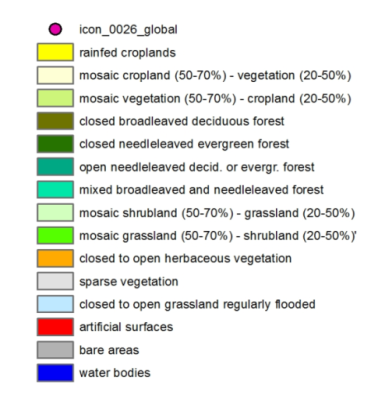
\includegraphics{../tex/extracted-media/media/image2.png}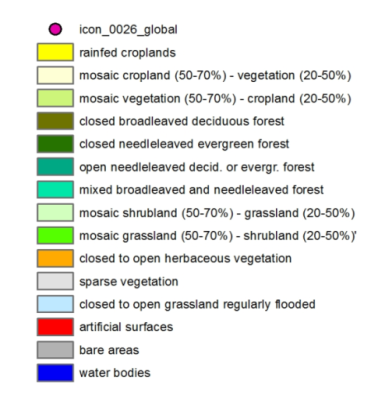
\includegraphics{../tex/extracted-media/media/image2.png} fields (that is, the total number of tile/attribute pairs, defined in octet 13) with indices (ITN, IAN) with the following meaning (IAN = \{1,\ldots, NAT(ITN)\}):

1,1 First tile -- first attribute (e.g. unmodified)

\ldots. \ldots.\\
1,NAT(1) First tile -- NAT of first tile (last, e.g. snow-covered) attribute

2,1 Second tile -- first attribute (e.g. unmodified)

\ldots. \ldots.\\
2,NAT(2) Second tile -- NAT of second tile (last, e.g. snow-covered) attribute

. .\\
. .

NUT,1 NUT tile -- first attribute (e.g. unmodified)

\ldots. ....\\
NUT,NAT(NUT) NUT tile -- NAT of last tile (last) attribute

A single tile/attribute index (ITN, IAN) with spatial tile index ITN (1,\ldots,NUT) and attribute A(IAN) with IAN = (1,\ldots,NAT(ITN)) is represented in the template. All NT partitions are linked by the normalization formula, which states that the sum of all partitions must be equal to a normalization term (N = 1 for fractions and N = 100 for percentage) on each point of the grid.

The fields "tile class" and "tile fraction" must be provided in order to obtain the tile structure of each grid point. Note that the field ``tile fraction'' is time-dependent in the case of defined attributes, whereas the field ``tile class'' is not affected by attributes (NT = NUT).

(2) For more information, see Part B, GRIB Attachment IV.

(3) Hours greater than 65534 will be coded as 65534.

\emph{\textbf{\\
}}

\emph{\textbf{Product definition template 4.56 -- individual ensemble forecast, control and perturbed, at a horizontal level or in a horizontal layer at a point in time for spatio-temporal changing tile parameters}}

\emph{Note: This template is deprecated. Template 4.59 should be used instead.}

Octet No. Contents

10 Parameter category (see Code table 4.1)

11 Parameter number (see Code table 4.2)

12 Tile classification (see Code table 4.242)

13 Total number (NT) of tile/attribute pairs (see Notes 1 and 2)

14 Number of used spatial tiles (NUT) (see Notes 1 and 2)

15 Tile index (ITN = \{1,\ldots, NUT\}) (see Note 1)

16 Number of used tile attributes (NAT) for tile ITN (see Note 1)

17 Attribute of tile (see Code table 4.241)) (A = \{A(1),\ldots, A(NAT(ITN))\}) (see Note 1)

18 Type of generating process (see Code table 4.3)

19 Background generating process identifier (defined by originating centre)

20 Analysis or forecast generating process identifier (defined by originating centre)

21--22 Hours of observational data cut-off after reference time (see Note 3)

23 Minutes of observational data cut-off after reference time

24 Indicator of unit of time range (see Code table 4.4)

25--28 Forecast time in units defined by octet 24

29 Type of first fixed surface (see Code table 4.5)

30 Scale factor of first fixed surface

31--34 Scaled value of first fixed surface

35 Type of second fixed surface (see Code table 4.5)

36 Scale factor of second fixed surface

37--40 Scaled value of second fixed surface

41 Perturbation number

42 Number of forecasts in ensemble

Notes:

(1) See Note 1 under product definition template 4.55.

(2) For more information, see Part B, GRIB Attachment IV.

(3) Hours greater than 65534 will be coded as 65534.

\emph{\textbf{\\
}}

\emph{\textbf{Product definition template 4.57 -- analysis or forecast at a horizontal level or in a horizontal layer\\
at a point in time for atmospheric chemical constituents based on a distribution function}}

Octet No. Contents

10 Parameter category (see Code table 4.1)

11 Parameter number (see Code table 4.2)

12--13 Atmospheric chemical constituent type (see Code table 4.230)

14--15 Number of modes (N) of distribution (see Note 1)

16--17 Mode number (l)

18--19 Type of distribution function (see Code table 4.240)

20 Number of following function parameters (Np), defined by type given in octets 18--19 (Type of\\
distribution function)

\emph{Repeat the following 5 octets for the number of function parameters (n = 1,} \emph{Np), if Np \textgreater{} 0}

21+5(n--1) List of scale factor of fixed distribution function parameter (p1--pNp), defined by type of distribution in octets 18--19

(22+5(n--1))--(25+5(n--1)) List of scaled value of fixed distribution function parameter (p1--pNp), defined by type of distribution in octets 18--19

21+5Np Type of generating process (see Code table 4.3)

22+5Np Background generating process identifier (defined by originating centre)

23+5Np Analysis or forecast generating process identifier (defined by originating centre)

(24+5Np)--(25+5Np) Hours of observational data cut-off after reference time (see Note 2)

26+5Np Minutes of observational data cut-off after reference time

27+5Np Indicator of unit of time range (see Code table 4.4)

(28+5Np)--(31+5Np) Forecast time in units defined by the previous octet

32+5Np Type of first fixed surface (see Code table 4.5)

33+5Np Scale factor of first fixed surface

(34+5Np)--(37+5Np) Scaled value of first fixed surface

38+5Np Type of second fixed surface (see Code table 4.5)

39+5Np Scale factor of second fixed surface

(40+5Np)--(43+5Np) Scaled value of second fixed surface

Notes:

(1) If Number of modes (N) \textgreater{} 1, then between x N fields with mode number l = 1, \ldots, N define the distribution function. x is the number of variable parameters in the distribution function.

(2) Hours greater than 65534 will be coded as 65534.

(3) For more information, see Part B, GRIB Attachment III.

\emph{\textbf{\\
}}

\emph{\textbf{Product definition template 4.58 -- individual ensemble forecast, control and perturbed, at\\
a horizontal level or in a horizontal layer at a point in time for\\
atmospheric chemical constituents based on a distribution\\
function}}

Octet No. Contents

10 Parameter category (see Code table 4.1)

11 Parameter number (see Code table 4.2)

12--13 Atmospheric chemical constituent type (see Code table 4.230)

14--15 Number of modes (N) of distribution (see Note 1)

16--17 Mode number (l)

18--19 Type of distribution function (see Code table 4.240)

20 Number of following function parameters (Np), defined by type given in octets 18--19 (Type of\\
distribution function)

\emph{Repeat the following 5 octets for the number of function parameters (n = 1,} \emph{Np), if Np \textgreater{} 0}

21+5(n--1) List of scale factor of fixed distribution function parameter (p1--pNp), defined by type of distribution in octets 18--19

(22+5(n--1))--(25+5(n--1)) List of scaled value of fixed distribution function parameter (p1--pNp), defined by type of distribution in octets 18--19

21+5Np Type of generating process (see Code table 4.3)

22+5Np Background generating process identifier (defined by originating centre)

23+5Np Analysis or forecast generating process identifier (defined by originating centre)

(24+5Np)--(25+5Np) Hours of observational data cut-off after reference time (see Note 2)

26+5Np Minutes of observational data cut-off after reference time

27+5Np Indicator of unit of time range (see Code table 4.4)

(28+5Np)--(31+5Np) Forecast time in units defined by the previous octet

32+5Np Type of first fixed surface (see Code table 4.5)

33+5Np Scale factor of first fixed surface

(34+5Np)--(37+5Np) Scaled value of first fixed surface

38+5Np Type of second fixed surface (see Code table 4.5)

39+5Np Scale factor of second fixed surface

(40+5Np)--(43+5Np) Scaled value of second fixed surface

44+5Np Type of ensemble forecast (see Code table 4.6)

45+5Np Perturbation number

46+5Np Number of forecasts in ensemble

Notes:

(1) If Number of modes (N) \textgreater{} 1, then between x N fields with mode number l = 1, \ldots, N define the distribution function. x is the number of variable parameters in the distribution function.

(2) Hours greater than 65534 will be coded as 65534.

(3) For more information, see Part B, GRIB Attachment III.

\emph{\textbf{Product definition template 4.59 -- individual ensemble forecast, control and perturbed, at\\
a horizontal level or in a horizontal layer at a point in time for\\
spatio-temporal changing tile parameters}}

Octet No. Contents

10 Parameter category (see Code table 4.1)

11 Parameter number (see Code table 4.2)

12 Tile classification (see Code table 4.242)

\emph{(continued)}

\emph{\\
(Product definition template 4.59 -- continued)}

Octet No. Contents

13 Total number (NT) of tile/attribute pairs (see Notes 1 and 2)

14 Number of used spatial tiles (NUT) (see Notes 1 and 2)

15 Tile index (ITN = \{1,\ldots, NUT\}) (see Note 1)

16 Number of used tile attributes (NAT) for tile ITN (see Note 1)

17 Attribute of tile (see Code table 4.241)) (A = \{A(1),\ldots, A(NAT(ITN))\}) (see Note 1)

18 Type of generating process (see Code table 4.3)

19 Background generating process identifier (defined by originating centre)

20 Analysis or forecast generating process identifier (defined by originating centre)

21--22 Hours of observational data cut-off after reference time (see Note 3)

23 Minutes of observational data cut-off after reference time

24 Indicator of unit of time range (see Code table 4.4)

25--28 Forecast time in units defined by octet 24

29 Type of first fixed surface (see Code table 4.5)

30 Scale factor of first fixed surface

31--34 Scaled value of first fixed surface

35 Type of second fixed surface (see Code table 4.5)

36 Scale factor of second fixed surface

37--40 Scaled value of second fixed surface

41 Type of ensemble forecast (see Code table 4.6)

42 Perturbation number

43 Number of forecasts in ensemble

Notes:

(1) See Note 2 under product definition template 4.55.

(2) For more information, see Part B, GRIB Attachment IV.

(3) Hours greater than 65534 will be coded as 65534.

\emph{\textbf{Product definition template 4.60 -- individual ensemble reforecast, control and perturbed, at a}} \emph{\textbf{horizontal level or in a horizontal layer at a point in time}}

Octet No. Contents

10 Parameter category (see Code table 4.1)

11 Parameter number (see Code table 4.2)

12 Type of generating process (see Code table 4.3)

13 Background generating process identifier (defined by originating centre)

14 Analysis or forecast generating process identifier (defined by originating centre)

15--16 Hours of observational data cut-off after reference time (see Note 1)

17 Minutes of observational data cut-off after reference time

18 Indicator of unit of time range (see Code table 4.4)

19--22 Forecast time in units defined by octet 18

23 Type of first fixed surface (see Code table 4.5)

24 Scale factor of first fixed surface

25--28 Scaled value of first fixed surface

29 Type of second fixed surface (see Code table 4.5)

30 Scale factor of second fixed surface

\emph{(continued)}

\emph{\\
(Product definition template 4.60 -- continued)}

Octet No. Contents

31--34 Scaled value of second fixed surface

35 Type of ensemble forecast (see Code table 4.6)

36 Perturbation number

37 Number of forecasts in ensemble

38--39 Year of model version date (see Note 2)

40 Month of model version date

41 Day of model version date

42 Hour of model version date

43 Minute of model version date

44 Second of model version date

Notes:

(1) Hours greater than 65534 will be coded as 65534.

(2) This is the date when the reforecast is produced with a particular version of the model.

\emph{\textbf{Product definition template 4.61 -- individual ensemble reforecast, control and perturbed, at a horizontal level or in a horizontal layer, in a continuous or non-continuous time interval}}

Octet No. Contents

10 Parameter category (see Code table 4.1)

11 Parameter number (see Code table 4.2)

12 Type of generating process (see Code table 4.3)

13 Background generating process identifier (defined by originating centre)

14 Forecast generating process identifier (defined by originating centre)

15--16 Hours after reference time of data cut-off (see Note 1)

17 Minutes after reference time of data cut-off

18 Indicator of unit of time range (see Code table 4.4)

19--22 Forecast time in units defined by octet 18 (see Note 2)

23 Type of first fixed surface (see Code table 4.5)

24 Scale factor of first fixed surface

25--28 Scaled value of first fixed surface

29 Type of second fixed surface (see Code table 4.5)

30 Scale factor of second fixed surface

31--34 Scaled value of second fixed surface

35 Type of ensemble forecast (see Code table 4.6)

36 Perturbation number

37 Number of forecasts in ensemble

38--39 Year of model version date (see Note 3)

40 Month of model version date

41 Day of model version date

42 Hour of model version date

43 Minute of model version date

44 Second of model version date

45--46 Year of end of overall time interval

47 Month of end of overall time interval

\emph{(continued)}

\emph{\\
(Product definition template 4.61 -- continued)}

Octet No. Contents

48 Day of end of overall time interval

49 Hour of end of overall time interval

50 Minute of end of overall time interval

51 Second of end of overall time interval

52 n -- number of time range specifications describing the time intervals used to calculate the\\
statistically processed field

53--56 Total number of data values missing in statistical process

\emph{57--68 Specification of the outermost (or only) time range over which statistical processing is done}

57 Statistical process used to calculate the processed field from the field at each time increment during\\
the time range (see Code table 4.10)

58 Type of time increment between successive fields used in the statistical processing\\
(see Code table 4.11)

59 Indicator of unit of time for time range over which statistical processing is done (see Code table 4.4)

60--63 Length of the time range over which statistical processing is done, in units defined by the previous\\
octet

64 Indicator of unit of time for the increment between the successive fields used (see Code table 4.4)

65--68 Time increment between successive fields, in units defined by the previous octet (see Notes 4 and 5)

\emph{69--nn These octets are included only if n\textgreater1, where nn = 56 + 12 x n}

69--80 As octets 57 to 68, next innermost step of processing

81--nn Additional time range specifications, included in accordance with the value of n. Contents as octets\\
57 to 68, repeated as necessary

Notes:

(1) Hours greater than 65534 will be coded as 65534.

(2) The reference time in section 1 and the forecast time together define the beginning of the overall time interval.

(3) This is the date when the reforecast is produced with a particular version of the model.

(4) An increment of zero means that the statistical processing is the result of a continuous (or near continuous) process, not the processing of a number of discrete samples. Examples of such continuous processes are the temperatures measured by analogue maximum and minimum thermometers or thermographs, and the rainfall measured by a raingauge.

(5) The reference and forecast times are successively set to their initial values plus or minus the increment, as defined by the type of time increment (one of octets 51, 63, 75 ...). For all but the innermost (last) time range, the next inner range is then processed using these reference and forecast times as the initial reference and forecast times.

\emph{\textbf{\\
}}

\emph{\textbf{Product definition template 4.67 -- average, accumulation and/or extreme values or other statistically processed values at a horizontal level or in a horizontal layer in a continuous or non-continuous time interval for atmospheric chemical constituents based on a distribution function}}

Octet No. Contents

10 Parameter category (see Code table 4.1)

11 Parameter number (see Code table 4.2)

12--13 Atmospheric chemical constituent type (see Code table 4.230)

14--15 Number of modes (N) of distribution (see Note 1)

16--17 Mode number (l)

18--19 Type of distribution function (see Code table 4.240 and Note 2)

20 Number of following function parameters (Np), defined by type given in octets 18--19 (Type of\\
distribution function)

\emph{Repeat the following 5 octets for the number of function parameters (n = 1, Np), if Np \textgreater{} 0}

21+5(n--1) List of scale factor of fixed distribution function parameter (p1--pNp), defined by type of distribution in octets 18--19

(22+5(n--1))--(25+5(n--1)) List of scaled value of fixed distribution function parameter (p1--pNp), defined by type of distribution in octets 18--19

21+5Np Type of generating process (see Code table 4.3)

22+5Np Background generating process identifier (defined by originating centre)

23+5Np Analysis or forecast generating process identifier (defined by originating centre)

(24+5Np)--(25+5Np) Hours of observational data cut-off after reference time (see Note 3)

26+5Np Minutes of observational data cut-off after reference time

27+5Np Indicator of unit of time range (see Code table 4.4)

(28+5Np)--(31+5Np) Forecast time in units defined by the previous octet (see Note 4)

32+5Np Type of first fixed surface (see Code table 4.5)

33+5Np Scale factor of first fixed surface

(34+5Np)--(37+5Np) Scaled value of first fixed surface

38+5Np Type of second fixed surface (see Code table 4.5)

39+5Np Scale factor of second fixed surface

(40+5Np)--(43+5Np) Scaled value of second fixed surface

(44+5Np)--(45+5Np) Year

(46+5Np) Month

(47+5Np) Day

(48+5Np) Hour

(49+5Np) Minute

(50+5Np) Second

(51+5Np) n -- number of time range specifications describing the time intervals used to calculate the statistically processed field

(52+5Np)--(55+5Np) Total number of data values missing in statistical process

\emph{(56+5Np)--(67+5Np) Specification of the outermost (or only) time range over which statistical processing is done}

(56+5Np) Statistical process used to calculate the processed field from the field at each time increment during the time range (see Code table 4.10)

(57+5Np) Type of time increment between successive fields used in the statistical processing (see Code table 4.11)

(58+5Np) Indicator of unit of time for time range over which statistical processing is done (see Code table 4.4)

(59+5Np)--(62+5Np) Length of the time range over which statistical processing is done, in units defined by the previous octet

\emph{(continued)}

\emph{\\
(Product definition template 4.67 -- continued)}

Octet No. Contents

(63+5Np) Indicator of unit of time for the increment between the successive fields used (see Code table~4.4)

(64+5Np)--(67+5Np) Time increment between successive fields, in units defined by the previous octet (see Notes 5 and 6)

\emph{(68+5Np)--nn These octets are included only if n \textgreater{} 1, where nn =} (55+5Np) \emph{+ 12 x n}

(68+5Np)--(79+5Np) As octets (56+5Np) to (67+5Np), next innermost step of processing

(80+5Np)--nn Additional time range specifications, included in accordance with the value of n. Contents as octets (56+5Np) to (67+5Np), repeated as necessary

Notes:

(1) If Number of modes (N) \textgreater{} 1, then between x N fields with mode number l = 1, \ldots, N define the distribution function. x is the number of variable parameters in the distribution function.

(2) For more information, see Part B, GRIB Attachment III.

(3) Hours greater than 65534 will be coded as 65534.

(4) The reference time in section 1 and the forecast time together define the beginning of the overall time interval.

(5) An increment of zero means that the statistical processing is the result of a continuous (or near continuous) process, not the processing of a number of discrete samples. Examples of such continuous processes are the temperatures measured by analogue maximum and minimum thermometers or thermographs, and the rainfall measured by a raingauge.

(6) The reference and forecast times are successively set to their initial values plus or minus the increment, as defined by the type of time increment. For all but the innermost (last) time range, the next inner range is then processed using these reference and forecast times as the initial reference and forecast times.

\emph{\textbf{Product definition template 4.68 -- individual ensemble forecast, control and perturbed, at a horizontal level or in a horizontal layer in a continuous or non-continuous time interval for atmospheric chemical constituents based on a distribution function}}

Octet No. Contents

10 Parameter category (see Code table 4.1)

11 Parameter number (see Code table 4.2)

12--13 Atmospheric chemical constituent type (see Code table 4.230)

14--15 Number of modes (N) of distribution (see Note 1)

16--17 Mode number (l)

18--19 Type of distribution function (see Code table 4.240 and Note 2)

20 Number of following function parameters (Np), defined by type given in octets 18--19 (Type of\\
distribution function)

\emph{Repeat the following 5 octets for the number of function parameters (n = 1, Np), if Np \textgreater{} 0}

21+5(n--1) List of scale factor of fixed distribution function parameter (p1--pNp), defined by type of distribution in octets 18--19

(22+5(n--1))--(25+5(n--1)) List of scaled value of fixed distribution function parameter (p1--pNp), defined by type of distribution in octets 18--19

21+5Np Type of generating process (see Code table 4.3)

22+5Np Background generating process identifier (defined by originating centre)

23+5Np Analysis or forecast generating process identifier (defined by originating centre)

(24+5Np)--(25+5Np) Hours of observational data cut-off after reference time (see Note 3)

26+5Np Minutes of observational data cut-off after reference time

27+5Np Indicator of unit of time range (see Code table 4.4)

\emph{(continued)}

\emph{\\
(Product definition template 4.68 -- continued)}

Octet No. Contents

(28+5Np)--(31+5Np) Forecast time in units defined by the previous octet (see Note 4)

32+5Np Type of first fixed surface (see Code table 4.5)

33+5Np Scale factor of first fixed surface

(34+5Np)--(37+5Np) Scaled value of first fixed surface

38+5Np Type of second fixed surface (see Code table 4.5)

39+5Np Scale factor of second fixed surface

(40+5Np)--(43+5Np) Scaled value of second fixed surface

44+5Np Type of ensemble forecast (see Code table 4.6)

45+5Np Perturbation number

46+5Np Number of forecasts in ensemble

(47+5Np)--(48+5Np) Year

(49+5Np) Month

(50+5Np) Day

(51+5Np) Hour

(52+5Np) Minute

(53+5Np) Second

(54+5Np) n -- number of time range specifications describing the time intervals used to calculate the statistically processed field

(55+5Np)--(58+5Np) Total number of data values missing in statistical process

\emph{(59+5Np)--(70+5Np) Specification of the outermost (or only) time range over which statistical processing is done}

(59+5Np) Statistical process used to calculate the processed field from the field at each time increment during the time range (see Code table 4.10)

(60+5Np) Type of time increment between successive fields used in the statistical processing (see Code table 4.11)

(61+5Np) Indicator of unit of time for time range over which statistical processing is done (see Code table 4.4)

(62+5Np)--(65+5Np) Length of the time range over which statistical processing is done, in units defined by the previous octet

(66+5Np) Indicator of unit of time for the increment between the successive fields used (see Code table~4.4)

(67+5Np)--(70+5Np) Time increment between successive fields, in units defined by the previous octet (see Notes 5 and 6)

\emph{(71+5Np)--nn These octets are included only if n \textgreater{} 1, where nn = (58+5Np) + 12 x n}

(71+5Np)--(82+5Np) As octets (59+5Np) to (70+5Np), next innermost step of processing

(83+5Np)--nn Additional time range specifications, included in accordance with the value of n. Contents as octets (59+5Np) to (70+5Np), repeated as necessary

Notes:

(1) If Number of modes (N) \textgreater{} 1, then between x N fields with mode number l = 1, \ldots, N define the distribution function. x is the number of variable parameters in the distribution function.

(2) For more information, see Part B, GRIB Attachment III.

(3) Hours greater than 65534 will be coded as 65534.

(4) The reference time in section 1 and the forecast time together define the beginning of the overall time interval.

(5) An increment of zero means that the statistical processing is the result of a continuous (or near continuous) process, not the processing of a number of discrete samples. Examples of such continuous processes are the temperatures measured by analogue maximum and minimum thermometers or thermographs, and the rainfall measured by a raingauge.

(6) The reference and forecast times are successively set to their initial values plus or minus the increment, as defined by the type of time increment. For all but the innermost (last) time range, the next inner range is then processed using these reference and forecast times as the initial reference and forecast times.

\emph{\textbf{Product definition template 4.70 -- post-processing analysis or forecast at a horizontal level or in a horizontal layer at a point in time}}

Octet No. Contents

10 Parameter category (see Code table 4.1)

11 Parameter number (see Code table 4.2)

12--13 Input process identifier (see Note 1)

14--15 Input originating centre (see Common Code table C--11 and Note 2)

16 Type of post-processing (see Note 3)

17 Type of generating process (see Code table 4.3)

18 Background generating process identifier (defined by originating centre)

19 Analysis or forecast generating process identifier (defined by originating centre)

20--21 Hours of observational data cut-off after reference time (see Note 4)

22 Minutes of observational data cut-off after reference time

23 Indicator of unit of time range (see Code table 4.4)

24--27 Forecast time in units defined by octet 23

28 Type of first fixed surface (see Code table 4.5)

29 Scale factor of first fixed surface

30--33 Scaled value of first fixed surface

34 Type of second fixed surface (see Code table 4.5)

35 Scale factor of second fixed surface

36--39 Scaled value of second fixed surface

Notes:

(1) The input process identifier shall have the value of the ``analysis or forecast process identifier'' of the original GRIB message used as input of the post-processing.

(2) The input originating centre shall have the value of the ``originating centre'' of the original GRIB message used as input of the post-processing.

(3) This identifies which post-processing technique was used. This is defined by the originating centre.

(4) Hours greater than 65534 will be coded as 65534.

\emph{\textbf{Product definition template 4.71 -- post-processing individual ensemble forecast, control and perturbed, at a horizontal level or in a horizontal layer at a point in time}}

Octet No. Contents

10 Parameter category (see Code table 4.1)

11 Parameter number (see Code table 4.2)

12--13 Input process identifier (see Note 1)

14--15 Input originating centre (see Common Code table C--11 and Note 2)

16 Type of post-processing (see Note 3)

17 Type of generating process (see Code table 4.3)

18 Background generating process identifier (defined by originating centre)

19 Forecast generating process identifier (defined by originating centre)

20--21 Hours after reference time of data cut-off (see Note 4)

22 Minutes after reference time of data cut-off

23 Indicator of unit of time range (see Code table 4.4)

24--27 Forecast time in units defined by octet 23

28 Type of first fixed surface (see Code table 4.5)

29 Scale factor of first fixed surface

\emph{(continued)}

\emph{\\
(Product definition template 4.71 -- continued)}

Octet No. Contents

30--33 Scaled value of first fixed surface

34 Type of second fixed surface (see Code table 4.5)

35 Scale factor of second fixed surface

36--39 Scaled value of second fixed surface

40 Type of ensemble forecast (see Code table 4.6)

41 Perturbation number

42 Number of forecasts in ensemble

Notes:

(1) The input process identifier shall have the value of the ``analysis or forecast process identifier'' of the original GRIB message used as input of the post-processing.

(2) The input originating centre shall have the value of the ``originating centre'' of the original GRIB message used as input of the post-processing.

(3) This identifies which post-processing technique was used. This is defined by the originating centre.

(4) Hours greater than 65534 will be coded as 65534.

\emph{\textbf{Product definition template 4.72 -- post-processing average, accumulation, extreme values or other statistically processed values at a horizontal level or in a horizontal layer in a continuous or non-continuous time interval}}

Octet No. Contents

10 Parameter category (see Code table 4.1)

11 Parameter number (see Code table 4.2)

12--13 Input process identifier (see Note 1)

14--15 Input originating centre (see Common Code table C--11 and Note 2)

16 Type of post-processing (see Note 3)

17 Type of generating process (see Code table 4.3)

18 Background generating process identifier (defined by originating centre)

19 Analysis or forecast generating process identifier (defined by originating centre)

20--21 Hours after reference time of data cut-off (see Note 4)

22 Minutes after reference time of data cut-off

23 Indicator of unit of time range (see Code table 4.4)

24--27 Forecast time in units defined by octet 23 (see Note 5)

28 Type of first fixed surface (see Code table 4.5)

29 Scale factor of first fixed surface

30--33 Scaled value of first fixed surface

34 Type of second fixed surface (see Code table 4.5)

35 Scale factor of second fixed surface

36--39 Scaled value of second fixed surface

40--41 Year

42 Month

43 Day

44 Hour

45 Minute

46 Second

47 n -- number of time range specifications describing the time intervals used to calculate the statistically\\
processed field

48--51 Total number of data values missing in statistical process

\emph{(continued)}

\emph{\\
(Product definition template 4.72 -- continued)}

Octet No. Contents

\emph{52--63 Specification of the outermost (or only) time range over which statistical}\\
\emph{processing is done}

52 Statistical process used to calculate the processed field from the field at each time increment\\
during the time range (see Code table 4.10)

53 Type of time increment between successive fields used in the statistical processing (see Code\\
table 4.11)

54 Indicator of unit of time for time range over which statistical processing is done (see Code\\
table 4.4)

55--58 Length of the time range over which statistical processing is done, in units defined by the\\
previous octet

59 Indicator of unit of time for the increment between the successive fields used (see Code\\
table 4.4)

60--63 Time increment between successive fields, in units defined by the previous octet (see Notes 6\\
and 7)

\emph{64--nn These octets are included only if n \textgreater{} 1, where nn = 51 + 12 x n}

64--75 As octets 52 to 63, next innermost step of processing

76--nn Additional time range specifications, included in accordance with the value of n. Contents as\\
octets 52 to 63, repeated as necessary

Notes:

(1) The input process identifier shall have the value of the ``analysis or forecast process identifier'' of the original GRIB message used as input of the post-processing.

(2) The input originating centre shall have the value of the ``originating centre'' of the original GRIB message used as input of the post-processing.

(3) This identifies which post-processing technique was used. This is defined by the originating centre.

(4) Hours greater than 65534 will be coded as 65534.

(5) The reference time in section 1 and the forecast time together define the beginning of the overall time interval.

(6) An increment of zero means that the statistical processing is the result of a continuous (or near continuous) process, not the processing of a number of discrete samples. Examples of such continuous processes are the temperatures measured by analogue maximum and minimum thermometers or thermographs, and the rainfall measured by a raingauge.

(7) The reference and forecast times are successively set to their initial values plus or minus the increment, as defined by the type of time increment (one of octets 63, 65, 77, ...). For all but the innermost (last) time range, the next inner range is then processed using these reference and forecast times as the initial reference and forecast times.

\emph{\textbf{Product definition template 4.73 -- post-processing individual ensemble forecast, control and perturbed, at a horizontal level or in a horizontal layer, in a continuous or non-continuous time interval}}

Octet No. Contents

10 Parameter category (see Code table 4.1)

11 Parameter number (see Code table 4.2)

12--13 Input process identifier (see Note 1)

14--15 Input originating centre (see Common Code table C--11 and Note 2)

16 Type of post-processing (see Note 3)

17 Type of generating process (see Code table 4.3)

18 Background generating process identifier (defined by originating centre)

19 Forecast generating process identifier (defined by originating centre)

20--21 Hours after reference time of data cut-off (see Note 4)

22 Minutes after reference time of data cut-off

23 Indicator of unit of time range (see Code table 4.4)

\emph{(continued)}

\emph{\\
(Product definition template 4.73 -- continued)}

Octet No. Contents

24--27 Forecast time in units defined by octet 23 (see Note 5)

28 Type of first fixed surface (see Code table 4.5)

29 Scale factor of first fixed surface

30--33 Scaled value of first fixed surface

34 Type of second fixed surface (see Code table 4.5)

35 Scale factor of second fixed surface

36--39 Scaled value of second fixed surface

40 Type of ensemble forecast (see Code table 4.6)

41 Perturbation number

42 Number of forecasts in ensemble

43--44 Year of end of overall time interval

45 Month of end of overall time interval

46 Day of end of overall time interval

47 Hour of end of overall time interval

48 Minute of end of overall time interval

49 Second of end of overall time interval

50 n -- number of time range specifications describing the time intervals used to calculate the\\
statistically processed field

51--54 Total number of data values missing in statistical process

\emph{55--66 Specification of the outermost (or only) time range over which statistical}\\
\emph{processing is done}

55 Statistical process used to calculate the processed field from the field at each time increment\\
during the time range (see Code table 4.10)

56 Type of time increment between successive fields used in the statistical processing (see Code\\
table 4.11)

57 Indicator of unit of time for time range over which statistical processing is done (see Code\\
table 4.4)

58--61 Length of the time range over which statistical processing is done, in units defined by the\\
previous octet

62 Indicator of unit of time for the increment between the successive fields used (see Code\\
table 4.4)

63--66 Time increment between successive fields, in units defined by the previous octet (see Notes 6 and 7)

\emph{67--nn These octets are included only if n \textgreater{} 1, where nn = 54 + 12 x n}

67--78 As octets 55 to 66, next innermost step of processing

79--nn Additional time range specifications, included in accordance with the value of n. Contents as\\
octets 55 to 66, repeated as necessary

Notes:

(1) The input process identifier shall have the value of the ``analysis or forecast process identifier'' of the original GRIB message used as input of the post-processing.

(2) The input originating centre shall have the value of the ``originating centre'' of the original GRIB message used as input of the post-processing.

(3) This identifies which post-processing technique was used. This is defined by the originating centre.

(4) Hours greater than 65534 will be coded as 65534.

(5) The reference time in section 1 and the forecast time together define the beginning of the overall time interval.

(6) An increment of zero means that the statistical processing is the result of a continuous (or near continuous) process, not the processing of a number of discrete samples. Examples of such continuous processes are the temperatures measured by analogue maximum and minimum thermometers or thermographs, and the rainfall measured by a raingauge.

\emph{(continued)}

\emph{\\
(Product definition template 4.73 -- continued)}

(7) The reference and forecast times are successively set to their initial values plus or minus the increment, as defined by the type of time increment (one of octets 56, 68, 80, ...). For all but the innermost (last) time range, the next inner range is then processed using these reference and forecast times as the initial reference and forecast times.

\begin{quote}
\emph{\textbf{Product definition template 4.91 -- categorical forecasts at a horizontal level or in a horizontal layer in a continuous or non-continuous time interval}}
\end{quote}

Octet No. Contents

10 Parameter category (see Code table 4.1)

11 Parameter number (see Code table 4.2)

12 Type of generating process (see Code table 4.3)

13 Background generating process identifier (defined by originating centre)

14 Forecast generating process identifier (defined by originating centre)

15--16 Hours after reference time of data cut-off (see Note 1)

17 Minutes after reference time of data cut-off

18 Indicator of unit of time range (see Code table 4.4)

19--22 Forecast time in units defined by octet 18 (see Note 2)

23 Type of first fixed surface (see Code table 4.5)

24 Scale factor of first fixed surface

25--28 Scaled value of first fixed surface

29 Type of second fixed surface (see Code table 4.5)

30 Scale factor of second fixed surface

31--34 Scaled value of second fixed surface

35 NC -- number of categories

\emph{36-- Repeat the following 12 octets for each category (i = 1,NC)}

(36+12(i--1)) Code figure

(37+12(i--1)) Type of interval for first and second limits (see Code table 4.91)

(38+12(i--1)) Scale factor of first limit

(39+12(i--1))--(42+12(i--1)) Scaled value of first limit

(43+12(i--1)) Scale factor of second limit

(44+12(i--1))--(47+12(i--1)) Scaled value of second limit

(48+12(NC--1))--(49+12(NC--1)) Year of end of overall time interval

(50+12(NC--1)) Month of end of overall time interval

(51+12(NC--1)) Day of end of overall time interval

(52+12(NC--1)) Hour of end of overall time interval

(53+12(NC--1)) Minute of end of overall time interval

(54+12(NC--1)) Second of end of overall time interval

(55+12(NC--1)) n -- number of time range specifications describing the time intervals\\
used to calculate the statistically processed field

(56+12(NC--1))--(59+12(NC--1)) Total number of data values missing in statistical process

\emph{60--71 Specification of the outermost (or only) time range over which}\\
\emph{statistical processing is done}

(60+12(NC--1)) Statistical process used to calculate the processed field from the field\\
at each time increment during the time range (see Code table 4.10)

(61+12(NC--1)) Type of time increment between successive fields used in the statistical\\
processing (see Code table 4.11)

(62+12(NC--1)) Indicator of unit of time for time range over which statistical processing\\
is done (see Code table 4.4)

\emph{(continued)}

\emph{\\
(Product definition template 4.91 -- continued)}

Octet No. Contents

(63+12(NC--1))--(66+12(NC--1)) Length of the time range over which statistical processing is done, in\\
units defined by the previous octet

(67+12(NC--1)) Indicator of unit of time for the increment between the successive fields\\
used (see Code table 4.4)

(68+12(NC--1))--(71+12(NC--1)) Time increment between successive fields, in units defined by the\\
previous octet (see Notes 3 and 4)

\emph{72--nn These octets are included only if n \textgreater{} 1, where nn = 72+12(n--1)}\\
\emph{+12(NC--1)}

(72+12(NC--1))--(83+12(NC--1)) As octets (60+12(NC--1)) to (71+12(NC--1)), next innermost step of\\
processing

(84+12(NC--1))--nn Additional time range specifications, included in accordance with the\\
value of n. Contents as octets (60+12(NC --1)) to (71+12(NC --1)),\\
repeated as necessary

Notes:

(1) Hours greater than 65534 will be coded as 65534.

(2) The reference time in section 1 and the forecast time together define the beginning of the overall time interval.

(3) An increment of zero means that the statistical processing is the result of a continuous (or near continuous) process, not the processing of a number of discrete samples. Examples of such continuous processes are the temperatures measured by analogue maximum and minimum thermometers or thermographs, and the rainfall measured by a raingauge.

(4) The reference and forecast times are successively set to their initial values plus or minus the increment, as defined by the type of time increment (one of octets (60+12(NC --1)), (73+12(NC --1)), (85+12(NC --1)), ...). For all but the innermost (last) time range, the next inner range is then processed using these reference and forecast times as the initial reference and forecast times.

\emph{\textbf{Product definition template 4.254 -- CCITT IA5 character string}}

Octet No. Contents

10 Parameter category (see Code table 4.1)

11 Parameter number (see Code table 4.2)

12--15 Number of characters

\emph{\textbf{Product definition template 4.1000 -- cross-section of analysis and forecast at a point in time}}

Preliminary note: This template is simply experimental, was not validated at the time of publication and should be used only for bilateral previously agreed tests.

Octet No. Contents

10 Parameter category (see Code table 4.1)

11 Parameter number (see Code table 4.2)

12 Type of generating process (see Code table 4.3)

13 Background generating process identifier (defined by originating centre)

14 Analysis or forecast generating process identifier (defined by originating centre)

15--16 Hours of observational data cut-off after reference time (see Note)

17 Minutes of observational data cut-off after reference time

18 Indicator of unit of time range (see Code table 4.4)

19--22 Forecast time in units defined by octet 18

Note: Hours greater than 65534 will be coded as 65534.

\emph{\textbf{\\
}}

\emph{\textbf{Product definition template 4.1001 -- cross-section of averaged or otherwise statistically\\
processed analysis or forecast over a range of time}}

Preliminary note: This template is simply experimental, was not validated at the time of publication and should be used only for bilateral previously agreed tests.

Octet No. Contents

10 Parameter category (see Code table 4.1)

11 Parameter number (see Code table 4.2)

12 Type of generating process (see Code table 4.3)

13 Background generating process identifier (defined by originating centre)

14 Analysis or forecast generating process identifier (defined by originating centre)

15--16 Hours of observational data cut-off after reference time (see Note 1)

17 Minutes of observational data cut-off after reference time

18 Indicator of unit of time range (see Code table 4.4)

19--22 Forecast time in units defined by octet 18

23--26 Total number of data values missing in the statistical process

27 Statistical process used to calculate the processed field from the field at each time incre-\\
ment during the time range (see Code table 4.10)

28 Type of time increment between successive fields used in the statistical processing (see\\
Code table 4.11)

29 Indicator of unit of time for time range over which statistical processing is done (see Code\\
table 4.4)

30--33 Length of the time range over which statistical processing is done, in units defined by the\\
previous octet

34 Indicator of unit of time for the increment between the successive fields used (see Code\\
table 4.4)

35--38 Time increment between successive fields, in units defined by the previous octet (see Note 2)

Notes:

(1) Hours greater than 65534 will be coded as 65534.

(2) An increment of zero means that the statistical processing is the result of a continuous (or near continuous) process, not the processing of a number of discrete samples. Examples of such continuous processes are the temperatures measured by analogue maximum and minimum thermometers or thermographs, and the rainfall measured by a raingauge.

\emph{\textbf{Product definition template 4.1002 -- cross-section of analysis and forecast, averaged or other-\\
wise statistically processed over latitude or longitude}}

Preliminary note: This template is simply experimental, was not validated at the time of publication and should be used only for bilateral previously agreed tests.

Octet No. Contents

10 Parameter category (see Code table 4.1)

11 Parameter number (see Code table 4.2)

12 Type of generating process (see Code table 4.3)

13 Background generating process identifier (defined by originating centre)

14 Analysis or forecast generating process identifier (defined by originating centre)

15--16 Hours of observational data cut-off after reference time (see Note)

17 Minutes of observational data cut-off after reference time

18 Indicator of unit of time range (see Code table 4.4)

19--22 Forecast time in units defined by octet 18

23 Horizontal dimension processed (see Code table 4.220)

\emph{(continued)}

\emph{\\
(Product definition template 4.1002 -- continued)}

Octet No. Contents

24 Treatment of missing data (e.g. below ground) (see Code table 4.221)

25 Type of statistical processing (see Code table 4.10)

26--29 Start of range

30--33 End of range

34--35 Number of values

Note: Hours greater than 65534 will be coded as 65534.

\emph{\textbf{Product definition template 4.1100 -- Hovmöller-type grid with no averaging or other statistical\\
processing}}

Preliminary note: This template is simply experimental, was not validated at the time of publication and should be used only for bilateral previously agreed tests.

Octet No. Contents

10 Parameter category (see Code table 4.1)

11 Parameter number (see Code table 4.2)

12 Type of generating process (see Code table 4.3)

13 Background generating process identifier (defined by originating centre)

14 Analysis or forecast generating process identifier (defined by originating centre)

15--16 Hours of observational data cut-off after reference time (see Note)

17 Minutes of observational data cut-off after reference time

18 Indicator of unit of time range (see Code table 4.4)

19--22 Forecast time in units defined by octet 18

23 Type of first fixed surface (see Code table 4.5)

24 Scale factor of first fixed surface

25--28 Scaled value of first fixed surface

29 Type of second fixed surface (see Code table 4.5)

30 Scale factor of second fixed surface

31--34 Scaled value of second fixed surface

Note: Hours greater than 65534 will be coded as 65534.

\emph{\textbf{Product definition template 4.1101 -- Hovmöller-type grid with averaging or other statistical\\
processing}}

Preliminary note: This template is simply experimental, was not validated at the time of publication and should be used only for bilateral previously agreed tests. (Octets 35--50 are very similar to octets 43--58 of product definition template 4.8, but the meaning of some fields differs slightly.)

Octet No. Contents

10 Parameter category (see Code table 4.1)

11 Parameter number (see Code table 4.2)

12 Type of generating process (see Code table 4.3)

13 Background generating process identifier (defined by originating centre)

14 Analysis or forecast generating process identifier (defined by originating centre)

15--16 Hours of observational data cut-off after reference time (see Note 1)

17 Minutes of observational data cut-off after reference time

18 Indicator of unit of time range (see Code table 4.4)

\emph{(continued)}

\emph{\\
(Product definition template 4.1101 -- continued)}

Octet No. Contents

19--22 Forecast time in units defined by octet 18 (see Note 2)

23 Type of first fixed surface (see Code table 4.5)

24 Scale factor of first fixed surface

25--28 Scaled value of first fixed surface

29 Type of second fixed surface (see Code table 4.5)

30 Scale factor of second fixed surface

31--34 Scaled value of second fixed surface

35--38 Total number of data values missing in the statistical process

39 Statistical process used to calculate the processed field from the field at each time incre-\\
ment during the time range (see Code table 4.10)

40 Type of time increment between successive fields used in the statistical processing (see\\
Code table 4.11)

41 Indicator of unit of time for time range over which statistical processing is done (see Code\\
table 4.4)

42--45 Length of the time range over which statistical processing is done, in units defined by the\\
previous octet

46 Indicator of unit of time for increment between the successive fields used (see Code\\
table 4.4)

47--50 Time increment between successive fields, in units defined by the previous octet (see\\
Note 3)

Notes:

(1) Hours greater than 65534 will be coded as 65534.

(2) Reference = reference time (section 1) + forecast range (PDT) + offset and increments from reference time (GDT).

(3) An increment of zero means that the statistical processing is the result of a continuous (or near continuous) process, not the processing of a number of discrete samples. Examples of such continuous processes are the temperatures measured by analogue maximum and minimum thermometers or thermographs, and the rainfall measured by a raingauge.

\textbf{TEMPLATE DEFINITIONS USED IN SECTION 5}

\emph{\textbf{Data representation template 5.0 -- Grid point data -- simple packing}}

Note: For most templates, details of the packing process are described in Regulation 92.9.4.

Octet No. Contents

12--15 Reference value (R) (IEEE 32-bit floating-point value)

16--17 Binary scale factor (E)

18--19 Decimal scale factor (D)

20 Number of bits used for each packed value for simple packing, or for each group reference\\
value for complex packing or spatial differencing

21 Type of original field values (see Code table 5.1)

Note: Negative values of E or D shall be represented according to Regulation 92.1.5.

\emph{\textbf{Data representation template 5.1 -- Matrix values at grid point -- simple packing}}

Preliminary note: This template was not validated at the time of publication and should be used with caution. Please report any use to WMO Secretariat (Observing and Information Systems Department) to assist for validation.

Note: For most templates, details of the packing process are described in Regulation 92.9.4

Octet No. Contents

12--21 Same as data representation template 5.0

22 0, no matrix bit maps present; 1--matrix bit maps present

23--26 Number of data values encoded in Section 7

27--28 NR -- first dimension (rows) of each matrix

29--30 NC -- second dimension (columns) of each matrix

31 First dimension coordinate value definition (Code table 5.2)

32 NC1 -- number of coefficients or values used to specify first dimension coordinate function

33 Second dimension coordinate value definition (Code table 5.2)

34 NC2 -- number of coefficients or values used to specify second dimension coordinate function

35 First dimension physical significance (Code table 5.3)

36 Second dimension physical significance (Code table 5.3)

37--(36+NC1x4) Coefficients to define first dimension coordinate values in functional form,\\
or the explicit coordinate values (IEEE 32-bit floating-point value)

(37+NC1x4)--(36+4(NC1+NC2)) Coefficients to define second dimension coordinate values in functional\\
form, or the explicit coordinate values (IEEE 32-bit floating-point value)

Notes:

(1) This form of representation enables a matrix of values to be depicted at each grid point; the two dimensions of the matrix may represent coordinates expressed in terms of two elemental parameters (e.g. direction and frequency for wave spectra). The numeric values of these coordinates, beyond that of simple subscripts, can be given in a functional form, or as a collection of explicit numbers.

(2) Some simple coordinate functional forms are tabulated in Code table 5.2. Where a more complex coordinate function applies, the coordinate values shall be explicitly denoted by the inclusion of the actual set of values rather than the coefficients. This shall be indicated by a code figure 0 from Code table 5.2; the number of explicit values coded shall be equal to the appropriate dimension of the matrix for which values are presented and they shall follow octet 36 in place of the coefficients.

(3) Matrix bit maps will be present only if indicated by octet 22. If present, there shall be one bit map for each grid point with data values, as defined by the primary bit map in Section 6, each of length (NR x NC) bits: a bit set to 1 will indicate a data element at the corresponding location within the matrix. Bit maps shall be represented end-to-end, without regard for octet boundaries; the last bit map shall, if necessary, be followed by bits set to zero to fill any partially used octet.

(4) Matrices restricted to scanning in the +i direction (left to right) and in the --j direction (top to bottom).

\emph{\textbf{Data representation template 5.2 -- Grid point data -- complex packing}}

Note: For most templates, details of the packing process are described in Regulation 92.9.4.

Octet No. Contents

12--21 Same as data representation template 5.0

22 Group splitting method used (see Code table 5.4)

23 Missing value management used (see Code table 5.5)

24--27 Primary missing value substitute

28--31 Secondary missing value substitute

32--35 NG -- number of groups of data values into which field is split

36 Reference for group widths (see Note 12)

37 Number of bits used for the group widths (after the reference value in octet 36 has been\\
removed)

38--41 Reference for group lengths (see Note 13)

42 Length increment for the group lengths (see Note 14)

43--46 True length of last group

47 Number of bits used for the scaled group lengths (after subtraction of the reference value\\
given in octets 38--41 and division by the length increment given in octet 42)

Notes:

(1) Group lengths have no meaning for row by row packing, where groups are coordinate lines (so the grid description section and possibly the bit-map section are enough); for consistency, associated field width and reference should then be encoded as 0.

(2) For row by row packing with a bit-map, there should always be as many groups as rows. In case of rows with only missing values, all associated descriptors should be coded as zero.

(3) Management of widths into a reference and increments, together with management of lengths as scaled incremental values, are intended to save descriptor size (which is an issue as far as compression gains are concerned).

(4) Management of explicitly missing values is an alternative to bit-map use within Section 6; it is intended to reduce the whole GRIB message size.

(5) There may be two types of missing value(s), such as to make a distinction between static misses (for instance, due to a land/sea mask) and occasional misses.

(6) As an extra option, substitute value(s) for missing data may be specified. If not wished (or not applicable), all bits should be set to 1 for relevant substitute value(s).

(7) If substitute value(s) are specified, type of content should be consistent with original field values (floating-point - and then IEEE 32-bit encoded-, or integer).

(8) If primary missing values are used, such values are encoded within appropriate group with all bits set to 1 at packed data level.

(9) If secondary missing values are used, such values are encoded within appropriate group with all bits set to 1, except the last one set to 0, at packed data level.

(10) A group containing only missing values (of either type) will be encoded as a constant group (null width, no associated data) and the group reference will have all bits set to 1 for primary type, and all bits set to 1, except the last bit set to 0, for secondary type.

(11) If necessary, group widths and/or field width of group references may be enlarged to avoid ambiguities between missing value indicator(s) and true data.

(12) The group width is the number of bits used for every value in a group.

(13) The group length (L) is the number of values in a group.

(14) The essence of the complex packing method is to subdivide a field of values into NG groups, where the values in each group have similar sizes. In this procedure, it is necessary to retain enough information to recover the group lengths upon decoding. The NG group lengths for any given field can be described by Ln = ref + Kn x len\_inc, n = 1, NG, where ref is given by octets 38--41 and len\_inc by octet 42. The NG values of K (the scaled group lengths) are stored in the data section, each with the number of bits specified by octet 47. Since the last group is a special case which may not be able to be specified by this relationship, the length of the last group is stored in octets 43--46.

(15) See data template 7.2 and associated Notes for complementary information.

\emph{\textbf{Data representation template 5.3 -- Grid point data -- complex packing and spatial differencing}}

Note: For most templates, details of the packing process are described in Regulation 92.9.4.

Octet No. Contents

12--47 Same as data representation template 5.2

48 Order of spatial differencing (see Code table 5.6)

49 Number of octets required in the data section to specify extra descriptors needed for spatial\\
differencing (octets 6--ww in data template 7.3)

Notes:

(1) Spatial differencing is a pre-processing before group splitting at encoding time. It is intended to reduce the size of sufficiently smooth fields, when combined with a splitting scheme as described in data representation template 5.2. At order 1, an initial field of values f is replaced by a new field of values g, where g\textsubscript{1} = f\textsubscript{1}, g\textsubscript{2} = f\textsubscript{2} -- f\textsubscript{1}, \ldots, g\textsubscript{n} = f\textsubscript{n} -- f\textsubscript{n--1}. At order 2, the field of values g is itself replaced by a new field of values h, where h\textsubscript{1} = f\textsubscript{1}, h\textsubscript{2} = f\textsubscript{2}, h\textsubscript{3} = g\textsubscript{3} -- g\textsubscript{2}, \ldots, h\textsubscript{n} = g\textsubscript{n} -- g\textsubscript{n--1}. To keep values positive, the overall minimum of the resulting field (either g\textsubscript{min} or h\textsubscript{min}) is removed. At decoding time, after bit string unpacking, the original scaled values are recovered by adding the overall minimum and summing up recursively.

(2) For differencing of order n, the first n values in the array that are not missing are set to zero in the packed array. These dummy values are not used in unpacking.

(3) See data template 7.3 and associated Notes for complementary information.

\emph{\textbf{Data representation template 5.4 -- Grid point data -- IEEE floating point data}}

Octet No. Contents

12 Precision (see Code table 5.7)

\emph{\textbf{Data representation template 5.40 -- Grid point data -- JPEG 2000 code stream format}}

Note: For most templates, details of the packing process are described in Regulation 92.9.4.

Octet No. Contents

12--15 Reference value (R) (IEEE 32-bit floating-point value)

16--17 Binary scale factor (E)

18--19 Decimal scale factor (D)

20 Number of bits required to hold the resulting scaled and referenced data values (i.e. depth\\
of the greyscale image) (see Note 2)

21 Type of original field values (see Code table 5.1)

22 Type of compression used (see Code table 5.40)

23 Target compression ratio, M:1 (with respect to the bit-depth specified in octet 20), when\\
octet 22 indicates lossy compression. Otherwise, set to missing (see Note 3)

Notes:

(1) The purpose of this template is to scale the grid point data to obtain the desired precision, if appropriate, and then subtract out the reference value from the scaled field as is done using data representation template 5.0. After this, the resulting grid point field can be treated as a greyscale image and is then encoded into the JPEG 2000 code stream format. To unpack the data field, the JPEG 2000 code stream is decoded back into an image, and the original field is obtained from the image data as described in Regulation 92.9.4, Note 4.

(2) The JPEG 2000 standard specifies that the bit-depth must be in the range of 1 to 38 bits.

(3) The compression ratio M:1 (e.g. 20:1) specifies that the encoded stream should be less than ((1/M) x depth x number of data points) bits, where depth is specified in octet 20 and the number of data points in octets 6--9 of the data representation section.

\emph{(continued)}

\emph{\\
(Data representation template 5.40 -- continued)}

(4) The order of the data points should remain as specified in the scanning mode flags (Flag table 3.4) set in the appropriate grid definition template, even though the JPEG 2000 standard specifies that an image is stored starting at the top left corner. Assuming that the encoding software is expecting the image data in raster order (left to right across rows for each row), users should set the image width to Ni (or Nx) and the height to Nj (or Ny) if bit 3 of the scanning mode flag equals 0 (adjacent points in i (x) order), when encoding the "image". If bit 3 of the scanning mode flags equals 1 (adjacent points in j (y) order), it may be advantageous to set the image width to Nj (or Ny) and the height to Ni (or Nx).

(5) This template should not be used when the data points are not available on a rectangular grid, such as occurs if some data points are bit-mapped out or if section 3 describes a quasi-regular grid. If it is necessary to use this template on such a grid, the data field can be treated as a one-dimensional image where the height is set to 1 and the width is set to the total number of data points specified in octets 6--9.

(6) Negative values of E or D shall be represented according to Regulation 92.1.5.

(7) JPEG 2000 should not be used for bit-mapped or quasi-regular grid data.

\emph{\textbf{Data representation template 5.41 -- Grid point data -- Portable Network Graphics (PNG) format}}

Note: For most templates, details of the packing process are described in Regulation 92.9.4.

Octet No. Contents

12--15 Reference value (R) (IEEE 32-bit floating-point value)

16--17 Binary scale factor (E)

18--19 Decimal scale factor (D)

20 Number of bits required to hold the resulting scaled and referenced data values (i.e. depth\\
of the image) (see Note 2)

21 Type of original field values (see Code table 5.1)

Notes:

(1) The purpose of this template is to scale the grid point data to obtain the desired precision, if appropriate, and then\\
subtract out the reference value from the scaled field, as is done using data representation template 5.0. After this, the resulting grid point field can be treated as an image and is then encoded into PNG format. To unpack the data field, the PNG stream is decoded back into an image, and the original field is obtained from the image data as described in Regulation 92.9.4, Note 4.

(2) PNG does not support all bit-depths in an image, so it is necessary to define which depths can be used and how they are to be treated. For greyscale images, PNG supports depths of 1, 2, 4, 8 or 16 bits. Red-Green-Blue (RGB) colour images can have depths of 8 or 16 bits with an optional alpha sample. Valid values for octet 20 can be:

1, 2, 4, 8, or 16 : Treat as greyscale image

24 : Treat as RGB colour image (each component having 8-bit depth)

32 : Treat as RGB w/ alpha sample colour image (each component having 8-bit depth)

(3) The order of the data points should remain as specified in the scanning mode flags (Flag table 3.4) set in the appropriate grid definition template, even though the PNG standard specifies that an image is stored starting at the top left corner and scans each row from left to right, starting with the top row. Users should set the image width to Ni (or Nx) and the height to Nj (or Ny) if bit 3 of the scanning mode flag equals 0 (adjacent points in i (x) order), when encoding the "image". If bit 3 of the scanning mode flags equals 1 (adjacent points in j (y) order), it may be advantageous to set the image width to Nj (or Ny) and the height to Ni (or Nx).

(4) This template should not be used when the data points are not available on a rectangular grid, such as occurs if some data points are bit-mapped out or if section 3 describes a quasi-regular grid. If it is necessary to use this template on such a grid, the data field can be treated as a one-dimensional image where the height is set to 1 and the width is set to the total number of data points specified in octets 6--9.

(5) Negative values of E or D shall be represented according to Regulation 92.1.5.

\emph{\textbf{Data representation template 5.42 -- Grid point and spectral data -- CCSDS recommended lossless\\
compression}}

Preliminary note: For most templates, details of the packing process are described in regulation 92.9.4.

This template is only valid for the Consultative Committee for Space Data Systems Recommendation for Space Data System Standards\emph{, Lossless Data Compression,} CCSDS 121.0-B-2, Blue Book, May 2012.

Octet No. Contents

12--15 Reference value (R) (IEEE 32-bit floating-point value)

16--17 Binary scale factor (E)

18--19 Decimal scale factor (D)

20 Number of bits required to hold the resulting scaled and referenced data values (see Note 1)

21 Type of original field values (see Code table 5.1)

22 CCSDS compression options mask (see Note 3)

23 Block size

24--25 Reference sample interval

Notes:

(1) The intent of this template is to scale the grid point data to obtain the desired precision, if appropriate, and then subtract the reference value from the scaled field, as is done using data representation template 5.0. After this, the resulting grid point field can be treated as a greyscale image and encoded into the CCSDS recommended standard for lossless data compression code stream format. To unpack the data field, the CCSDS recommended standard for lossless data compression code stream is decoded back into an image, and the original field is obtained from the image data as described in regulation 92.9.4, Note 4.

(2) The Consultative Committee for Space Data Systems (CCSDS) recommended standard for lossless data compression is the standard used by space agencies for the compression of scientific data transmitted from satellites and other space instruments. CCSDS recommended standard for lossless data compression is a very fast predictive compression algorithm based on the extended-Rice algorithm. It uses Golomb--Rice codes for entropy coding. The sequence of prediction errors is divided into blocks. Each block is compressed using a two-pass algorithm. In the first pass, the best coding method for the whole block is determined. In the second pass, the output of the marker of the selected coding method is encoded as ancillary information along with prediction errors.

The coding methods include:

\begin{itemize}
\item
  \begin{quote}
  Golomb--Rice codes of a chosen rank
  \end{quote}
\item
  \begin{quote}
  Unary code for transformed pairs of prediction errors
  \end{quote}
\item
  \begin{quote}
  Fixed-length natural binary code if the block is found to be incompressible
  \end{quote}
\item
  \begin{quote}
  Signalling to the decoder empty block if all prediction errors are zeroes
  \end{quote}
\end{itemize}

(3) Library flags governing data type, and storage and processing parameters. For further information, see Rosenhauer, Mathis. ``Flags.'' libaec -- Adaptive Entropy Coding library. German Climate Computing Centre (Deutsches Klimarechenzentrum, DKRZ), 12 May 2016. Web. 13 June 2016.

\textless{}\href{http://gitlab.dkrz.de/k202009/libaec/blob/v0.3.3/README.md\#flags}{http:/gitlab.dkrz.de/k202009/libaec/blob/v0.3.3/README.md\#flags}\textgreater.

\emph{\textbf{Data representation template 5.50 -- Spectral data -- simple packing}}

Note: For most templates, details of the packing process are described in Regulation 92.9.4.

Octet No. Contents

12--15 Reference value (R) (IEEE 32-bit floating-point value)

16--17 Binary scale factor (E)

18--19 Decimal scale factor (D)

20 Number of bits used for each packed value (field width)

21--24 Real part of (0.0) coefficient (IEEE 32-bit floating-point value)

\emph{(continued)}

\emph{\\
(Product definition template 5.50 -- continued)}

Notes:

(1) Removal of the real part of (0.0) coefficient from packed data is intended to reduce the variability of the coefficients, in order to improve packing accuracy.

(2) For some spectral representations, the (0.0) coefficient represents the mean value of the parameter represented.

(3) Negative values of E or D shall be represented according to Regulation 92.1.5.

\emph{\textbf{Data representation template 5.51 -- Spherical harmonics data -- complex packing}}

Note: For most templates, details of the packing process are described in Regulation 92.9.4.

Octet No. Contents

12--20 Same as data representation template 5.50

21--24 P -- Laplacian scaling factor (expressed in 10\textsuperscript{--6} units)

25--26 J\textsubscript{S} -- pentagonal resolution parameter of the unpacked subset (see Note 1)

27--28 K\textsubscript{S} -- pentagonal resolution parameter of the unpacked subset (see Note 1)

29--30 M\textsubscript{S} -- pentagonal resolution parameter of the unpacked subset (see Note 1)

31--34 T\textsubscript{S} -- total number of values in the unpacked subset (see Note 1)

35 Precision of the unpacked subset (see Code table 5.7)

Notes:

(1) The unpacked subset is a set of values defined in the same way as the full set of values (on a spectrum limited to J\textsubscript{S}, K\textsubscript{S} and M\textsubscript{S}), but on which scaling and packing are not applied. Associated values are stored in octets 6 onwards\\
of Section 7.

(2) The remaining coefficients are multiplied by (n x (n+1))\textsuperscript{P}, scaled and packed. The operator associated with this multiplication is derived from the Laplacian operator on the sphere.

(3) The retrieval formula for a coefficient of wave number n is then:

Y = (R + X x 2\textsuperscript{E}) x10\textsuperscript{--D} x (n x (n+1))\textsuperscript{--P} where X is the packed scaled value associated with the coefficient.

\emph{\textbf{Data representation template 5.61 -- Grid point data -- simple packing with logarithm pre-processing}}

Preliminary note: This template is experimental, was not validated at the time of publication and should be used only for bilateral previously agreed tests.

Octet No. Contents

12--15 Reference value (R) (IEEE 32-bit floating-point value)

16--17 Binary scale factor (E)

18--19 Decimal scale factor (D)

20 Number of bits used for each packed value

21--24 Pre-processing parameter (B) (IEEE 32-bit floating-point value)

Notes:

(1) This template is appropriately designed for data sets with all non-negative values and a wide variability range (more then 5 orders of magnitude). It must not be used for data sets with negative values or smaller variability range.

(2) A logarithm pre-processing algorithm is used to fit the variability range into one or two order of magnitudes before using the simple packing algorithm. It requires a parameter (B) to assure that all values passed to the logarithm function are positive. Thus scaled values are Z = ln (Y+B), where Y are the original values, ln is the natural logarithm (or Napierian) function and B is chosen so that Y+B \textgreater{} 0.

(3) Best practice follows for choosing the B pre-processing parameter.

\begin{quote}
(a) If the data set minimum value is positive, B can be safely put to zero.

(b) If the data set minimum is zero, all values must be scaled to become greater than zero and B can be equal to the minimum positive value in the data set.
\end{quote}

(4) Data shall be packed using data template 7.

\emph{\textbf{Data representation template 5.200 -- Grid point data -- run length packing with level values}}

Octet No. Contents

12 Number of bits used for each packed value in the run length packing with level value

13--14 MV -- maximum value within the levels that are used in the packing

15--16 MVL -- maximum value of level (predefined)

17 Decimal scale factor of representative value of each level

18--(19+2(lv--1)) List of MVL scaled representative values of each level from lv = 1 to MVL

\_\_\_\_\_\_\_\_\_\_\_\_

\textbf{TEMPLATE DEFINITIONS USED IN SECTION 7}

\emph{\textbf{Data template 7.0 -- Grid point data -- simple packing}}

Note: For most templates, details of the packing process are described in Regulation 92.9.4.

Octet No. Contents

6--nn Binary data values -- binary string, with each (scaled) data value

\emph{\textbf{Data template 7.1 -- Matrix values at grid point -- simple packing}}

Preliminary note: This template was not validated at the time of publication and should be used with caution. Please report any use to WMO Secretariat to assist for validation.

Note: For most templates, details of the packing process are described in Regulation 92.9.4.

Octet No. Contents

6--nn Binary data values -- binary string, with each (scaled) data value

Note: Group descriptors mentioned above may not be physically present; if associated field width is 0.

\emph{\textbf{Data template 7.2 -- Grid point data -- complex packing}}

Note: For most templates, details of the packing process are described in Regulation 92.9.4.

Octet No. Contents

6--xx NG group reference values (X1 in the decoding formula), each of which is encoded using\\
the number of bits specified in octet 20 of data representation template 5.0. Bits set to zero\\
shall be appended as necessary to ensure this sequence of numbers ends on an octet\\
boundary

{[}xx+1{]}--yy NG group widths, each of which is encoded using the number of bits specified in octet 37\\
of data representation template 5.2. Bits set to zero shall be appended as necessary to\\
ensure this sequence of numbers ends on an octet boundary

{[}yy+1{]}--zz NG scaled group lengths, each of which is encoded using the number of bits specified in\\
octet 47 of data representation template 5.2. Bits set to zero shall be appended as neces-\\
sary to ensure this sequence of numbers ends on an octet boundary (see Note 14 of data\\
representation template 5.2)

{[}zz+1{]}--nn Packed values (X2 in the decoding formula), where each value is a deviation from its respec-\\
tive group reference value

Notes:

(1) Group descriptors mentioned above may not be physically present; if associated field width is 0.

(2) Group lengths have no meaning for row by row packing; for consistency, associated field width should then be encoded as 0. So no specific test for row by row case is mandatory at decoding software level to handle encoding/decoding of group descriptors.

(3) Scaled group lengths, if present, are encoded for each group. But the true last group length (unscaled) should be taken from data representation template.

(4) For groups with a constant value, associated field width is 0, and no incremental data are physically present.

\emph{\textbf{Data template 7.3 -- Grid point data -- complex packing and spatial differencing}}

Note: For most templates, details of the packing process are described in Regulation 92.9.4.

Octet No. Contents

6--ww First value(s) of original (undifferenced) scaled data values, followed by the overall minimum\\
of the differences. The number of values stored is 1 greater than the order of differentiation,\\
and the field width is described at octet 49 of data representation template 5.3 (see Note 1)

{[}ww+1{]}--xx NG group reference values (X1 in the decoding formula), each of which is encoded using the num-\\
ber of bits specified in octet 20 of data representation template 5.0. Bits set to zero shall be\\
appended where necessary to ensure this sequence of numbers ends on an octet boundary

{[}xx+1{]}--nn Same as for data representation template 7.2

Notes:

(1) Referring to the notation in Note 1 of data representation template 5.3, at order 1, the values stored in octets 6--ww are g\textsubscript{1} and g\textsubscript{min}. At order 2, the values stored are h\textsubscript{1}, h\textsubscript{2}, and h\textsubscript{min}.

(2) Extra descriptors related to spatial differencing are added before the splitting descriptors, to reflect the separation between the two approaches. It enables to share software parts between cases with and without spatial differencing.

(3) The position of overall minimum after initial data values is a choice that enables less software management.

(4) Overall minimum will be negative in most cases. First bit should indicate the sign: 0 if positive, 1 if negative.

\emph{\textbf{Data template 7.4 -- Grid point data -- IEEE floating point data}}

Octet No. Contents

6--nn Binary data values

\emph{\textbf{Data template 7.40 -- Grid point data -- JPEG 2000 code stream format}}

Note: For most templates, details of the packing process are described in Regulation 92.9.4.

Octet No. Contents

6--nn JPEG 2000 code stream as described in Part 1 of the JPEG 2000 standard\\
(ISO/IEC 15444-1:2000)

Note: For simplicity, image data should be packed specifying a single component (i.e. greyscale image) instead of a multi-\\
component colour image.

\emph{\textbf{Data template 7.41 -- Grid point data -- Portable Network Graphics (PNG) format}}

Note: For most templates, details of the packing process are described in Regulation 92.9.4.

Octet No. Contents

6--nn PNG encoded image

Note: If octet 20 of data representation template 5.41 specifies the data are packed into either 1, 2, 4, 8, or 16 bits, then encode the "image" as a greyscale image. If octet 20 specifies 24 bits, encode the "image" as a Red-Green-Blue (RGB) colour image with 8-bit depth for each colour component, and finally if octet 20 is 32, encode the "image" as an RGB colour image with an alpha sample using 8-bit depth for each of the four components.

\emph{\textbf{Data template 7.42 -- Grid point and spectral data -- CCSDS recommended lossless compression}}

Octet No. Contents

6--nn CCSDS recommended standard for lossless data compression code stream

\emph{\textbf{\\
}}

\emph{\textbf{Data template 7.50 -- Spectral data -- simple packing}}

Note: For most templates, details of the packing process are described in Regulation 92.9.4.

Octet No. Contents

6--nn Binary data values -- binary string, with each (scaled) data value

\emph{\textbf{Data template 7.51 -- Spherical harmonics -- complex packing}}

Note: For most templates, details of the packing process are described in Regulation 92.9.4.

Octet No. Contents

6--(5+IxT\textsubscript{S}) Data values from the unpacked subset (IEEE floating-point values on I octets)

(6+IxT\textsubscript{S})--nn Binary data values -- binary string, with each (scaled) data value out of the unpacked subset

Notes:

(1) Values ordering within the unpacked subset is defined according to the source of grid definition associated with the data.

(2) Number of octets associated with each value of the unpacked subset (I) is defined in Code table 5.7, according to the actual value in octet 35 of data representation template 5.51.

(3) Values ordering within the packed data is done according to the source of grid definition, skipping the values processed in the unpacked subset.

\_\_\_\_\_\_\_\_\_\_\_
